\documentclass[a4paper]{article}

\def\npart {IB}
\def\nterm {Lent}
\def\nyear {2016}
\def\nlecturer {G.\ Moore}
\def\ncourse {Numerical Analysis}

\usepackage{myheader}

\begin{document}
\maketitle
{\small
\noindent\textbf{Polynomial approximation}\\
Interpolation by polynomials. Divided differences of functions and relations to derivatives. Orthogonal polynomials and their recurrence relations. Least squares approximation by polynomials. Gaussian quadrature formulae. Peano kernel theorem and applications.\hspace*{\fill} [6]

\vspace{10pt}
\noindent\textbf{Computation of ordinary differential equations}\\
Euler's method and proof of convergence. Multistep methods, including order, the root condition and the concept of convergence. Runge-Kutta schemes. Stiff equations and A-stability.\hspace*{\fill} [5]

\vspace{10pt}
\noindent\textbf{Systems of equations and least squares calculations}\\
LU triangular factorization of matrices. Relation to Gaussian elimination. Column pivoting. Factorizations of symmetric and band matrices. The Newton-Raphson method for systems of non-linear algebraic equations. QR factorization of rectangular matrices by Gram-Schmidt, Givens and Householder techniques. Application to linear least squares calculations.\hspace*{\fill} [5]}

\tableofcontents
\setcounter{section}{-1}
\section{Introduction}
Numerical analysis is the study of algorithms. There are many problems we would like algorithms to solve. In this course, we will tackle the problems of polynomial approximation, solving ODEs and solving linear equations. These are all problems that frequently arise when we do (applied) maths.

In general, there are two things we are concerned with --- accuracy and speed. Accuracy is particularly important in the cases of polynomial approximation and solving ODEs, since we are trying approximate things. We would like to make good approximations of the solution with relatively little work. On the other hand, in the case of solving linear equations, we are more concerned with speed --- our solutions will be exact (up to numerical errors due to finite precision of calculations), but we would like to solve it quickly. We might have to deal with huge systems, and we don't want the computation time to grow too quickly.

In the past, this was an important subject, since they had no computers. The algorithms had to be implemented by hand. It was thus very important to find some practical and efficient methods of computing things, or else it would take them forever to calculate what they wanted. So we wanted quick algorithms that give reasonably accurate results.

Nowadays, this is still an important subject. While we have computers that are much faster at computation, we still want our programs to be fast. We would also want to get really accurate results, since we might be using them to, say, send our rocket to the Moon. Moreover, with more computational power, we might sacrifice efficiency for some other desirable properties. For example, if we are solving for the trajectory of a particle, we might want the solution to satisfy the conservation of energy. This would require some much more complicated and slower algorithms that no one would have considered in the past. Nowadays, with computers, these algorithms become more feasible, and are becoming increasingly more popular.

\section{Polynomial interpolation}
Polynomials are nice. Writing down a polynomial of degree $n$ involves only $n + 1$ numbers. They are easy to evaluate, integrate and differentiate. So it would be nice if we can approximate things with polynomials. For simplicity, we will only deal with real polynomials.

\begin{notation}
  We write $P_n[x]$ for the real linear vector space of polynomials (with real coefficients) having degree $n$ or less.
\end{notation}
It is easy to show that $\dim (P_n[x]) = n + 1$.

\subsection{The interpolation problem}
The idea of polynomial interpolation is that we are given $n + 1$ distinct interpolation points $\{x_i\}_{i = 0}^n \subseteq \R$, and $n + 1$ data values $\{f_i\}_{i = 0}^n \subseteq \R$. The objective is to find a $p \in P_n[x]$ such that
\[
  p(x_i) = f_i\quad \text{for}\quad i = 0, \cdots, n.
\]
In other words, we want to fit a polynomial through the points $(x_i, f_i)$.

There are many situations where this may come up. For example, we may be given $n + 1$ actual data points, and we want to fit a polynomial through the points. Alternatively, we might have a complicated function $f$, and want to approximate it with a polynomial $p$ such that $p$ and $f$ agree on at least that $n + 1$ points.

The naive way of looking at this is that we try a polynomial
\[
  p(x) = a_n x^n + a_{n - 1}x^{n - 1} + \cdots + a_0,
\]
and then solve the system of equations
\[
  f_i = p(x_i) = a_n x_i^n + a_{n - 1}x_i^{n - 1} + \cdots + a_0.
\]
This is a perfectly respectable system of $n + 1$ equations in $n + 1$ unknowns. From linear algebra, we know that in general, such a system is not guaranteed to have a solution, and if the solution exists, it is not guaranteed to be unique.

That was not helpful. So our first goal is to show that in the case of polynomial interpolation, the solution exists and is unique.

\subsection{The Lagrange formula}
It turns out the problem is not too hard. You can probably figure it out yourself if you lock yourself in a room for a few days (or hours). In fact, we will come up with \emph{two} solutions to the problem.

The first is via the Lagrange cardinal polynomials. These are simple to state, and it is obvious that these work very well. However, practically, this is not the best way to solve the problem, and we will not talk about them much. Instead, we use this solution as a proof of existence of polynomial interpolations. We will then develop our second method on the assumption that polynomial interpolations exist, and find a better way of computing them.

\begin{defi}[Lagrange cardinal polynomials]
  The \emph{Lagrange cardinal polynomials} with respect to the interpolation points $\{x_i\}_{i = 0}^n$ are, for $k = 0, \cdots, n$,
  \[
    \ell_k (x) = \prod_{i = 0, i \not= k}^n \frac{x - x_i}{x_k - x_i}.
  \]
\end{defi}
Note that these polynomials have degree exactly $n$. The significance of these polynomials is we have $\ell_k(x_i) = 0$ for $i \not= k$, and $\ell_k(x_k) = 1$. In other words, we have
\[
  \ell_k(x_j) = \delta_{jk}.
\]
This is obvious from definition.

With these cardinal polynomials, we can immediately write down a solution to the interpolation problem.
\begin{thm}
  The interpolation problem has exactly one solution.
\end{thm}

\begin{proof}
  We define $p \in P_n[x]$ by
  \[
    p(x) = \sum_{k = 0}^n f_k \ell_k (x).
  \]
  Evaluating at $x_i$ gives
  \[
    p(x_j) = \sum_{k = 0}^n f_k \ell_k(x_j) = \sum_{k = 0}^n f_k \delta_{jk} = f_j.
  \]
  So we get existence.

  For uniqueness, suppose $p, q \in P_n[x]$ are solutions. Then the difference $r = p - q \in P_n[x]$ satisfies $r(x_j) = 0$ for all $j$, i.e.\ it has $n + 1$ roots. However, a non-zero polynomial of degree $n$ can have at most $n$ roots. So in fact $p - q$ is zero, i.e.\ $p = q$.
\end{proof}

While this \emph{works}, it is not ideal. If we one day decide we should add one more interpolation point, we would have to recompute all the cardinal polynomials, and that is not fun. Ideally, we would like some way to reuse our previous computations when we have new interpolation points.

\subsection{The Newton formula}
The idea of Newton's formula is as follows --- for $k = 0, \cdots, n$, we write $p_k \in P_k[x]$ for the polynomial that satisfies
\[
  p_k(x_i) = f_i\quad\text{for}\quad i = 0, \cdots, k.
\]
This is the unique degree-$k$ polynomial that satisfies the first $k + 1$ conditions, whose existence (and uniqueness) is guaranteed by the previous section. Then we can write
\[
  p(x) = p_n(x) = p_0(x) + (p_1(x) - p_0(x)) + \cdots + (p_n(x) - p_{n - 1}(x)).
\]
Hence we are done if we have an efficient way of finding the differences $p_k - p_{k - 1}$.

We know that $p_k$ and $p_{k - 1}$ agree on $x_0, \cdots, x_{k - 1}$. So $p_k - p_{k - 1}$ evaluates to $0$ at those points, and we must have
\[
  p_k(x) - p_{k - 1}(x) = A_k \prod_{i = 0}^{k - 1}(x - x_i),
\]
for some $A_k$ yet to be found out. Then we can write
\[
  p(x) = p_n(x) = A_0 + \sum_{k = 1}^n A_k \prod_{i = 0}^{k - 1} (x - x_i).
\]
This formula has the advantage that it is built up gradually from the interpolation points one-by-one. If we stop the sum at any point, we have obtained the polynomial that interpolates the data for the first $k$ points (for some $k$). Conversely, if we have a new data point, we just need to add a new term, instead of re-computing everything.

All that remains is to find the coefficients $A_k$. For $k = 0$, we know $A_0$ is the unique constant polynomial that interpolates the point at $x_0$, i.e.\ $A_0 = f_0$.

For the others, we note that in the formula for $p_k - p_{k - 1}$, we find that $A_k$ is the leading coefficient of $x^k$. But $p_{k - 1}(x)$ has no degree $k$ term. So $A_k$ must be the leading coefficient of $p_k$. So we have reduced our problem to finding the leading coefficients of $p_k$.

The solution to this is known as the \emph{Newton divided differences}. We first invent a new notation:
\[
  A_k = f[x_0, \cdots, x_k].
\]
Note that these coefficients depend only on the first $k$ interpolation points. Moreover, since the labelling of the points $x_0, \cdots, x_k$ is arbitrary, we don't have to start with $x_0$. In general, the coefficient
\[
  f[x_j, \cdots, x_k]
\]
is the leading coefficient of the unique $q \in P_{k - j}[x]$ such that $q(x_i) = f_i$ for $i = j, \cdots, k$.

While we do not have an explicit formula for what these coefficients are, we can come up with a recurrence relation for these coefficients.

\begin{thm}[Recurrence relation for Newton divided differences]
  For $0 \leq j < k \leq n$, we have
  \[
    f[x_j, \cdots, x_k] = \frac{f[x_{j + 1}, \cdots, x_k] - f[x_j, \cdots, x_{k - 1}]}{x_k - x_j}.
  \]
\end{thm}

\begin{proof}
  The key to proving this is to relate the interpolating polynomials. Let $q_0, q_1 \in P_{k - j - 1}[x]$ and $q_2 \in P_{k - j}$ satisfy
  \begin{align*}
    q_0(x_i) &= f_i & i &=j, \cdots, k - 1\\
    q_1(x_i) &= f_i & i &=j + 1, \cdots, k\\
    q_2(x_i) &= f_i & i &=j, \cdots, k
  \end{align*}
  We now claim that
  \[
    q_2(x) = \frac{x - x_j}{x_k - x_j} q_1(x) + \frac{x_k - x}{x_k - x_j} q_0(x).
  \]
  We can check directly that the expression on the right correctly interpolates the points $x_i$ for $i = j, \cdots, k$. By uniqueness, the two expressions agree. Since $f[x_j, \cdots, x_k$], $f[x_{j + 1}, \cdots, x_k]$ and $f[x_j, \cdots, x_{k - 1}]$ are the leading coefficients of $q_2, q_1, q_0$ respectively, the result follows.
\end{proof}
Thus the famous Newton divided difference table can be constructed
\begin{center}
  \begin{tabular}{cccccc}
    \toprule
    $x_i$ & $f_i$ & $f[*, *]$ & $f[*, *, *]$ & $\cdots$ & $f[*, \cdots,*]$\\
    \midrule
    $x_0$ & $f[x_0]$\\
    & & $f[x_0, x_1]$\\
    $x_1$ & $f[x_1]$ & & $f[x_0, x_1, x_2]$ \\
    & & $f[x_1, x_2]$ & & $\ddots$\\
    $x_2$ & $f[x_2]$ & & $f[x_2, x_3, x_4]$ & $\cdots$ & $f[x_0, x_1, \cdots, x_n]$\\
    & & $f[x_2, x_3]$ & & $\iddots$\\
    $x_3$ & $f[x_3]$ & & $\iddots$\\
    $\vdots$ & $\vdots$ & $\iddots$ &\\
    $x_n$ & $f[x_n]$\\
    \bottomrule
  \end{tabular}
\end{center} % beautify
From the first $n$ columns, we can find the $n + 1$th column using the recurrence relation above. The values of $A_k$ can then be found at the top diagonal, and this is all we really need. However, to compute this diagonal, we will need to compute everything in the table.

In practice, we often need not find the actual interpolating polynomial. If we just want to evaluate $p(\hat{x})$ at some new point $\hat{x}$ using the divided table, we can use \emph{Horner's scheme}, given by
\begin{alltt}
  S <- f[\(\mathtt{x\sb{0}}\),..., \(\mathtt{x\sb{n}}\)]
  for k = n - 1,..., 0
      S <- (\(\mathtt{\hat{x}}\) - \(\mathtt{x\sb{k}}\))S + f[\(\mathtt{x\sb{0}}\),..., \(\mathtt{x\sb{k}}\)]
  end\end{alltt}
This only takes $O(n)$ operations.

If an extra data point $\{x_{n + 1}, f_{n + 1}\}$ is added, then we only have to compute an extra diagonal $f[x_k, \cdots, x_{n + 1}]$ for $k =n, \cdots, 0$ in the divided difference table to obtain the new coefficient, and the old results can be reused. This requires $O(n)$ operations. This is less straightforward for Lagrange's method.

\subsection{A useful property of divided differences}
In the next couple of sections, we are interested in the error of polynomial interpolation. Suppose the data points come from $f_i = f(x_i)$ for some complicated $f$ we want to approximate, and we interpolate $f$ at $n$ data points $\{x_i\}_{i = 1}^n$ with $p_n$. How does the error $e_n(x) = f(x) - p_n(x)$ depend on $n$ and the choice of interpolation points?

At the interpolation point, the error is necessarily $0$, by definition of interpolation. However, this does not tell us anything about the error elsewhere.

Our ultimate objective is to bound the error $e_n$ by suitable multiples of the derivatives of $f$. We will do this in two steps. We first relate the derivatives to the divided differences, and then relate the error to the divided differences.

The first part is an easy result based on the following purely calculus lemma.
\begin{lemma}
  Let $g \in C^m[a, b]$ have a continuous $m$th derivative. Suppose $g$ is zero at $m + \ell$ distinct points. Then $g^{(m)}$ has at least $\ell$ distinct zeros in $[a, b]$.
\end{lemma}

\begin{proof}
  This is a repeated application of Rolle's theorem. We know that between every two zeros of $g$, there is at least one zero of $g' \in C^{m - 1}[a, b]$. So by differentiating once, we have lost at most $1$ zeros. So after differentiating $m$ times, $g^{(m)}$ has lost at most $m$ zeros. So it still has at least $\ell$ zeros.
\end{proof}

\begin{thm}
  Let $\{x_i\}_{i = 0}^n \in [a, b]$ and $f \in C^n[a, b]$. Then there exists some $\xi \in (a, b)$ such that
  \[
    f[x_0, \cdots, x_n] = \frac{1}{n!} f^{(n)}(\xi).
  \]
\end{thm}

\begin{proof}
  Consider $e = f - p_n \in C^n[a, b]$. This has at least $n + 1$ distinct zeros in $[a, b]$. So by the lemma, $e^{(n)} = f^{(n)} - p_n^{(n)}$ must vanish at some $\xi \in (a, b)$. But then $p_n^{(n)} = n! f[x_0, \cdots, x_n]$ constantly. So the result follows.
\end{proof}

\subsection{Error bounds for polynomial interpolation}
The actual error bound is not too difficult as well. It turns out the error $e = f - p_n$ is ``like the next term in the Newton's formula''. This vague sentence is made precise in the following theorem:
\begin{thm}
  Assume $\{x_i\}_{i = 0}^n \subseteq [a, b]$ and $f \in C[a, b]$. Let $\bar{x} \in [a, b]$ be a non-interpolation point. Then
  \[
    e_n(\bar{x}) = f[x_0, x_1, \cdots, x_n, \bar{x}] \omega(\bar{x}),
  \]
  where
  \[
    \omega(x) = \prod_{i = 0}^n (x - x_i).
  \]
\end{thm}
Note that we forbid the case where $\bar{x}$ is an interpolation point, since it is not clear what the expression $f[x_0, x_1, \cdots, x_n, \bar{x}]$ means. However, if $\bar{x}$ is an interpolation point, then both $e_n(\bar x)$ and $\omega(\bar{x})$ are zero, so there isn't much to say.

\begin{proof}
  We think of $\bar{x} = x_{n + 1}$ as a new interpolation point so that
  \[
    p_{n + 1}(x) - p_n(x) = f[x_0, \cdots, x_n, \bar{x}] \omega(x)
  \]
  for all $x \in R$. In particular, putting $x = \bar{x}$, we have $p_{n + 1}(\bar{x}) = f(\bar{x})$, and we get the result.
\end{proof}

Combining the two results, we find
\begin{thm}
  If in addition $f \in C^{n + 1}[a, b]$, then for each $x \in [a, b]$, we can find $\xi_x \in (a, b)$ such that
  \[
    e_n(x) = \frac{1}{(n + 1)!} f^{(n + 1)}(\xi_x) \omega(x)
  \]
\end{thm}

\begin{proof}
  The statement is trivial if $x$ is an interpolation point --- pick arbitrary $\xi_x$, and both sides are zero. Otherwise, this follows directly from the last two theorems.
\end{proof}

This is an exact result, which is not too useful, since there is no easy constructive way of finding what $\xi_x$ should be. Instead, we usually go for a bound. We introduce the max norm
\[
  \|g\|_{\infty} = \max_{t \in [a, b]} |g(t)|.
\]
This gives the more useful bound
\begin{cor}
  For all $x \in [a, b]$, we have
  \[
    |f(x) - p_n(x)| \leq \frac{1}{(n + 1)!} \|f^{(n + 1)}\|_{\infty} |\omega(x)|
  \]
\end{cor}

Assuming our function $f$ is fixed, this error bound depends only on $\omega(x)$, which depends on our choice of interpolation points. So can we minimize $\omega(x)$ in some sense by picking some clever interpolation points $\Delta = \{x_i\}_{i = 0}^n$? Here we will have $n$ fixed. So instead, we put $\Delta$ as the subscript. We can write our bound as
\[
  \|f - p_{\Delta}\|_{\infty} \leq \frac{1}{(n + 1)!} \|f^{(n + 1)}\|_{\infty} \|\omega_{\Delta}\|_{\infty}.
\]
So the objective is to find a $\Delta$ that minimizes $\|\omega_{\Delta}\|_{\infty}$.

For the moment, we focus on the special case where the interval is $[-1, 1]$. The general solution can be obtained by an easy change of variable.

For some magical reasons that hopefully will become clear soon, the optimal choice of $\Delta$ comes from the \emph{Chebyshev polynomials}.
\begin{defi}[Chebyshev polynomial]
  The \emph{Chebyshev polynomial} of degree $n$ on $[-1, 1]$ is defined by
  \[
    T_n(x) = \cos(n \theta),
  \]
  where $x = \cos \theta$ with $\theta\in [0, \pi]$.
\end{defi}
So given an $x$, we find the unique $\theta$ that satisfies $x = \cos \theta$, and then find $\cos (n \theta)$. This is in fact a polynomial in disguise, since from trigonometric identities, we know $\cos (n\theta)$ can be expanded as a polynomial in $\cos \theta$ up to degree $n$.

Two key properties of $T_n$ on $[-1, 1]$ are
\begin{enumerate}
  \item The maximum absolute value is obtained at
    \[
      X_k = \cos\left(\frac{\pi k}{n}\right)
    \]
    for $k = 0, \cdots, n$ with
    \[
      T_n(X_k) = (-1)^k.
    \]
  \item This has $n$ distinct zeros at
    \[
      x_k = \cos\left(\frac{2k - 1}{2n}\pi\right).
    \]
    for $k = 1, \cdots, n$.
\end{enumerate}
When plotted out, the polynomials look like this:
\begin{center}
  \begin{tikzpicture}[scale=2]
    \draw [->] (-1.5, 0) -- (1.5, 0) node [right] {$x$};
    \draw [->] (0, -1.5) -- (0, 1.5) node [above] {$T_4(x)$};

    \draw [mblue,domain=0:180, samples=40] plot [smooth] ({cos(\x)}, {cos(4*\x)});
    \draw [dashed] (-1, -1) rectangle (1, 1);
    \node at (-1, 0) [below] {$-1$};
    \node at (1, 0) [below] {$1$};
    \node at (0, 1) [anchor = south west] {$1$};
    \node at (0, -1) [left] {$-1$};
  \end{tikzpicture}
\end{center}
All that really matters about the Chebyshev polynomials is that the maximum is obtained at $n + 1$ distinct points with alternating sign. The exact form of the polynomial is not really important.

Notice there is an intentional clash between the use of $x_k$ as the zeros and $x_k$ as the interpolation points --- we will show these are indeed the optimal interpolation points.

We first prove a convenient recurrence relation for the Chebyshev polynomials:
\begin{lemma}[3-term recurrence relation]
  The Chebyshev polynomials satisfy the recurrence relations
  \[
    T_{n + 1}(x) = 2x T_n(x) - T_{n - 1}(x)
  \]
  with initial conditions
  \[
    T_0(x) = 1,\quad T_1(x) = x.
  \]
\end{lemma}

\begin{proof}
  \[
    \cos((n + 1) \theta) + \cos((n - 1)\theta) = 2\cos \theta \cos(n\theta).\qedhere
  \]
\end{proof}
This recurrence relation can be useful for many things, but for our purposes, we only use it to show that the leading coefficient of $T_n$ is $2^{n - 1}$ (for $n \geq 1$).

\begin{thm}[Minimal property for $n \geq 1$]
  On $[-1, 1]$, among all polynomials $p \in P_n[x]$ with leading coefficient $1$, $\frac{1}{2^{n - 1}} \|T_n\|$ minimizes $\|p\|_{\infty}$. Thus, the minimum value is $\frac{1}{2^{n - 1}}$.
\end{thm}

\begin{proof}
  We proceed by contradiction. Suppose there is a polynomial $q_n \in P_n$ with leading coefficient $1$ such that $\|q_n\|_{\infty} < \frac{1}{2^{n - 1}}$. Define a new polynomial
  \[
    r = \frac{1}{2^{n - 1}}T_n - q_n.
  \]
  This is, by assumption, non-zero.

  Since both the polynomials have leading coefficient $1$, the difference must have degree at most $n - 1$, i.e.\ $r \in P_{n - 1}[x]$. Since $\frac{1}{2^{n - 1}}T_n(X_k) = \pm \frac{1}{2^{n - 1}}$, and $|q_n(X_n)| < \frac{1}{2^{n - 1}}$ by assumption, $r$ alternates in sign between these $n + 1$ points. But then by the intermediate value theorem, $r$ has to have at least $n$ zeros. This is a contradiction, since $r$ has degree $n - 1$, and cannot be zero.
\end{proof}

\begin{cor}
  Consider
  \[
    w_\Delta = \prod_{i = 0}^n (x - x_i) \in P_{n + 1}[x]
  \]
  for any distinct points $\Delta = \{x_i\}_{i = 0}^n \subseteq [-1, 1]$. Then
  \[
    \min_{\Delta} \|\omega_{\Delta}\|_{\infty} = \frac{1}{2^n}.
  \]
  This minimum is achieved by picking the interpolation points to be the zeros of $T_{n + 1}$, namely
  \[
    x_k = \cos\left(\frac{2k + 1}{2n + 2} \pi\right), \quad k = 0, \cdots, n.
  \]
\end{cor}

\begin{thm}
  For $f \in C^{n + 1}[-1, 1]$, the Chebyshev choice of interpolation points gives
  \[
    \|f - p_n\|_{\infty} \leq \frac{1}{2^n} \frac{1}{(n + 1)!} \|f^{(n + 1)}\|_{\infty}.
  \]
\end{thm}
Suppose $f$ has as many continuous derivatives as we want. Then as we increase $n$, what happens to the error bounds? The coefficients involve dividing by an exponential \emph{and} a factorial. Hence as long as the higher derivatives of $f$ don't blow up too badly, in general, the error will tend to zero as $n \to \infty$, which makes sense.

The last two results can be easily generalized to arbitrary intervals $[a, b]$, and this is left as an exercise for the reader.

\section{Orthogonal polynomials}
It turns out the Chebyshev polynomials is just an example of a more general class of polynomials, known as \emph{orthogonal polynomials}. As in linear algebra, we can define a scalar product on the space of polynomials, and then find a basis of orthogonal polynomials of the vector space under this scalar product. We shall show that each set of orthogonal polynomials has a three-term recurrence relation, just like the Chebyshev polynomials.

\subsection{Scalar product}
The scalar products we are interested in would be generalization of the usual scalar product on Euclidean space,
\[
  \bra \mathbf{x}, \mathbf{y}\ket = \sum_{i = 1}^n x_i y_i.
\]
We want to generalize this to vector spaces of functions and polynomials. We will not provide a formal definition of vector spaces and scalar products on an abstract vector space. Instead, we will just provide some examples of commonly used ones.
\begin{eg}\leavevmode
  \begin{enumerate}
    \item Let $V = C^s[a, b]$, where $[a, b]$ is a finite interval and $s \geq 0$. Pick a weight function $w(x) \in C(a, b)$ such that $w(x) > 0$ for all $x \in (a, b)$, and $w$ is integrable over $[a, b]$. In particular, we allow $w$ to vanish at the end points, or blow up mildly such that it is still integrable.

      We then define the inner product to be
      \[
        \bra f, g\ket = \int_a^b w(x) f(x) d(x)\;\d x.
      \]
    \item We can allow $[a, b]$ to be infinite, e.g.\ $[0, \infty)$ or even $(-\infty, \infty)$, but we have to be more careful. We first define
      \[
        \bra f, g\ket = \int_a^b w(x) f(x) g(x) \;\d x
      \]
      as before, but we now need more conditions. We require that $\int_a^b w(x) x^n\;\d x$ to exist for all $n \geq 0$, since we want to allow polynomials in our vector space. For example, $w(x) = e^{-x}$ on $[0, \infty)$, works, or $w(x) = e^{-x^2}$ on $(-\infty, \infty)$. These are scalar products for $P_n[x]$ for $n \geq 0$, but we cannot extend this definition to all smooth functions since they might blow up too fast at infinity. We will not go into the technical details, since we are only interested in polynomials, and knowing it works for polynomials suffices.
    \item We can also have a discrete inner product, defined by
      \[
        \bra f, g\ket = \sum_{j = 1}^m w_j f(\xi_j) g(\xi_j)
      \]
      with $\{\xi_j\}_{j = 1}^m$ distinct points and $\{w_j\}_{j = 1}^m > 0$. Now we have to restrict ourselves a lot. This is a scalar product for $V = P_{m - 1}[x]$, but not for higher degrees, since a scalar product should satisfy $\bra f, f \ket > 0$ for $f \not= 0$. In particular, we cannot extend this to all smooth functions.
  \end{enumerate}
\end{eg}
With an inner product, we can define orthogonality.
\begin{defi}[Orthogonalilty]
  Given a vector space $V$ and an inner product $\bra \ph, \ph\ket$, two vectors $f, g \in V$ are \emph{orthogonal} if $\bra f, g\ket = 0$.
\end{defi}

\subsection{Orthogonal polynomials}
\begin{defi}[Orthogonal polynomial]
  Given a vector space $V$ of polynomials and inner product $\bra \ph, \ph\ket$, we say $p_n \in P_n[x]$ is the \emph{$n$th orthogonal polynomial} if
  \[
    \bra p_n, q\ket = 0\text{ for all }q \in P_{n - 1}[x].
  \]
  In particular, $\bra p_n, p_m\ket = 0$ for $n \not= m$.
\end{defi}

We said \emph{the} orthogonal polynomial, but we need to make sure such a polynomial has to be unique. It is clearly not unique, since if $p_n$ satisfies these relations, then so does $\lambda p_n$ for all $\lambda \not= 0$. For uniqueness, we need to impose some scaling. We usually do so by requiring the leading polynomial to be $1$, i.e.\ it is monic.

\begin{defi}[Monic polynomial]
  A polynomial $p \in P_n[x]$ is \emph{monic} if the coefficient of $x^n$ is $1$.
\end{defi}
In practice, most famous traditional polynomials are not monic. They have a different scaling imposed. Still, as long as we have \emph{some} scaling, we will have uniqueness.

We will not mess with other scalings, and stick to requiring them to be monic since this is useful for proving things.

\begin{thm}
  Given a vector space $V$ of functions and an inner product $\bra \ph, \ph \ket$, there exists a unique monic orthogonal polynomial for each degree $n \geq 0$. In addition, $\{p_k\}_{k = 0}^n$ form a basis for $P_n[x]$.
\end{thm}

\begin{proof}
  This is a big induction proof over both parts of the theorem. We induct over $n$. For the base case, we pick $p_0(x) = 1$, which is the only degree-zero monic polynomial.

  Now suppose we already have $\{p_n\}_{k = 0}^n$ satisfying the induction hypothesis.

  Now pick any monic $q_{n + 1} \in P_{n + 1}[x]$, e.g.\ $x^{n + 1}$. We now construct $p_{n + 1}$ from $q_{n + 1}$ by the Gram-Schmidt process. We define
  \[
    p_{n + 1} = q_{n + 1} - \sum_{k = 0}^n \frac{\bra q_{n + 1}, p_k\ket}{\bra p_k, p_k\ket} p_k.
  \]
  This is again monic since $q_{n + 1}$ is, and we have
  \[
    \bra p_{n + 1}, p_m \ket = 0
  \]
  for all $m \leq n$, and hence $\bra p_{n + 1}, p\ket = 0$ for all $p \in P_n[x] = \bra p_0, \cdots,p_n\ket$.

  To obtain uniqueness, assume both $p_{n + 1}, \hat{p}_{n + 1} \in P_{n + 1}[x]$ are both monic orthogonal polynomials. Then $r = p_{n + 1} - \hat{p}_{n + 1} \in P_n[x]$. So
  \[
    \bra r, r\ket = \bra r, p_{n + 1} - \hat{p}_{n + 1}\ket = \bra r, p_{n + 1}\ket - \bra r, \hat{p}_{n + 1}\ket = 0 - 0 = 0.
  \]
  So $r = 0$. So $p_{n + 1} = \hat{p}_{n - 1}$.

  Finally, we have to show that $p_0, \cdots, p_{n + 1}$ form a basis for $P_{n + 1}[x]$. Now note that every $p \in P_{n + 1}[x]$ can be written uniquely as
  \[
    p = cp_{n + 1} + q,
  \]
  where $q \in P_n[x]$. But $\{p_k\}_{k = 0}^n$ is a basis for $P_n[x]$. So $q$ can be uniquely decomposed as a linear combination of $p_0, \cdots, p_n$.

  Alternatively, this follows from the fact that any set of orthogonal vectors must be linearly independent, and since there are $n + 2$ of these vectors and $P_{n + 1}[x]$ has dimension $n + 2$, they must be a basis.
\end{proof}

In practice, following the proof naively is not the best way of producing the new $p_{n + 1}$. Instead, we can reduce a lot of our work by making a clever choice of $q_{n + 1}$.

\subsection{Three-term recurrence relation}
Recall that for the Chebyshev polynomials, we obtained a three-term recurrence relation for them using special properties of the cosine. It turns out these recurrence relations exist in general for orthogonal polynomials.

We start by picking $q_{n + 1} = xp_n$ in the previous proof. We now use the fact that
\[
  \bra xf, g\ket = \bra f, xg\ket.
\]
This is not necessarily true for arbitrary inner products, but for most sensible inner products we will meet in this course, this is true. In particular, it is clearly true for inner products of the form
\[
  \bra f, g\ket = \int w(x) f(x) g(x)\;\d x.
\]
Assuming this, we obtain the following theorem.
\begin{thm}
  Monic orthogonal polynomials are generated by
  \[
    p_{k + 1}(x) = (x - \alpha_k)p_k(x) - \beta_k p_{k - 1}(x)
  \]
  with initial conditions
  \[
    p_0 = 1,\quad p_1(x) = (x - \alpha_0) p_0,
  \]
  where
  \[
    \alpha_k = \frac{\bra x p_k, p_k\ket}{\bra p_k, p_k\ket},\quad \beta_k = \frac{\bra p_k, p_k\ket}{\bra p_{k - 1}, p_{k - 1}\ket}.
  \]
\end{thm}

\begin{proof}
  By inspection, the $p_1$ given is monic and satisfies
  \[
    \bra p_1, p_0\ket = 0.
  \]
  Using $q_{n + 1} = x p_n$ in the Gram-Schmidt process gives
  \begin{align*}
    p_{n + 1} &= xp_n - \sum_{k = 0}^n \frac{\bra x p_n, p_k\ket}{\bra p_k, p_k\ket} p_k\\
    p_{n + 1} &= xp_n - \sum_{k = 0}^n \frac{\bra p_n, x p_k\ket}{\bra p_k, p_k\ket} p_k\\
    \intertext{We notice that $\bra p_n, xp_k\ket$ and vanishes whenever $x p_k$ has degree less than $n$. So we are left with}
    &= xp_n - \frac{\bra x p_n, p_n\ket}{\bra p_n, p_n\ket}p_n - \frac{\bra p_n, xp_{n - 1}\ket}{\bra p_{n - 1}, p_{n - 1}\ket} p_{n - 1}\\
    &= (x - \alpha_n) p_n - \frac{\bra p_n, xp_{n - 1}\ket}{\bra p_{n - 1}, p_{n - 1}\ket} p_{n - 1}.
  \end{align*}
  Now we notice that $xp_{n - 1}$ is a monic polynomial of degree $n$ so we can write this as $x p_{n - 1} = p_n + q$. Thus
  \[
    \bra p_n, xp_{n - 1}\ket = \bra p_n, p_n + q\ket = \bra p_n, p_n\ket.
  \]
  Hence the coefficient of $p_{n - 1}$ is indeed the $\beta$ we defined.
\end{proof}

\subsection{Examples}
The four famous examples are the Legendre polynomials, Chebyshev polynomials, Laguerre polynomials and Hermite polynomials. We first look at how the Chebyshev polynomials fit into this framework.

Chebyshev is based on the scalar product defined by
\[
  \bra f, g\ket = \int_{-1}^1 \frac{1}{\sqrt{1 - x^2}} f(x) g(x)\;\d x.
\]
Note that the weight function blows up mildly at the end, but this is fine since it is still integrable.

This links up with
\[
  T_n (x) = \cos(n\theta)
\]
for $x = \cos \theta$ via the usual trigonometric substitution. We have
\begin{align*}
  \bra T_n, T_m \ket &= \int_0^\pi \frac{1}{\sqrt{1 - \cos^2 \theta}} \cos(n\theta) \cos (m\theta) \sin \theta \;\d \theta\\
  &= \int_0^\pi \cos(n\theta) \cos (m\theta)\;\d \theta\\
  &= 0\text{ if }m\not= n.
\end{align*}
The other orthogonal polynomials come from scalar products of the form
\[
  \bra f, g\ket = \int_a^b w(x) f(x) g(x)\;\d x,
\]
as described in the table below:
\begin{center}
  \begin{tabular}{ccc}
    \toprule
    Type & Range & Weight\\
    \midrule
    Legendre & $[-1, 1]$ & $1$\\
    Chebyshev & $[-1, 1]$ & $\frac{1}{\sqrt{1 - x^2}}$\\
    Laguerre & $[0, \infty)$ & $e^{-x}$\\
    Hermite & $(-\infty, \infty)$ & $e^{-x^2}$\\
    \bottomrule
  \end{tabular}
\end{center}
\subsection{Least-squares polynomial approximation}
If we want to approximate a function with a polynomial, polynomial interpolation might not be the best idea, since all we do is make sure the polynomial agrees with $f$ at certain points, and then hope it is a good approximation elsewhere. Instead, the idea is to choose a polynomial $p$ in $P_n[x]$ that ``minimizes the error''.

What exactly do we mean by minimizing the error? The error is defined as the function $f - p$. So given an appropriate inner product on the vector space of continuous functions, we want to minimize
\[
  \|f - p\|^2 = \bra f - p, f - p\ket.
\]
This is usually of the form
\[
  \bra f - p, f - p\ket = \int_a^b w(x) [f(x) - p(x)]^2 \;\d x,
\]
but we can also use alternative inner products such as
\[
  \bra f - p, f - p\ket = \sum_{j = 1}^m w_j [f(\xi_i) - p(\xi_i)]^2.
\]
Unlike polynomial interpolation, there is no guarantee that the approximation agrees with the function anywhere. Unlike polynomial interpolation, there is some guarantee that the total error is small (or as small as we can get, by definition). In particular, if $f$ is continuous, then the Weierstrass approximation theorem tells us the total error must eventually vanish.

Unsurprisingly, the solution involves the use of the orthogonal polynomials with respect to the corresponding inner products.
\begin{thm}
  If $\{p_n\}_{k = 0}^n$ are orthogonal polynomials with respect to $\bra \ph, \ph \ket$, then the choice of $c_k$ such that
  \[
    p = \sum_{k = 0}^n c_k p_k
  \]
  minimizes $\|f - p\|^2$ is given by
  \[
    c_k = \frac{\bra f, p_k\ket}{\|p_k\|^2},
  \]
  and the formula for the error is
  \[
    \|f - p\|^2 = \|f\|^2 - \sum_{k = 0}^n \frac{\bra f, p_k\ket^2}{\|p_k\|^2}.
  \]
\end{thm}
Note that the solution decouples, in the sense that $c_k$ depends only on $f$ and $p_k$. If we want to take one more term, we just need to compute an extra term, and not redo our previous work.

Also, we notice that the formula for the error is a positive term $\|f\|^2$ subtracting a lot of squares. As we increase $n$, we subtract more squares, and the error decreases. If we are lucky, the error tends to $0$ as we take $n \to \infty$. Even though we might not know how many terms we need in order to get the error to be sufficiently small, we can just keep adding terms until the computed error small enough (which is something we have to do anyway even if we knew what $n$ to take).

\begin{proof}
  We consider a general polynomial
  \[
    p = \sum_{k = 0}^n c_k p_k.
  \]
  We substitute this in to obtain
  \[
    \bra f - p, f - p\ket = \bra f, f\ket - 2 \sum_{k = 0}^n c_k \bra f, p_k\ket + \sum_{k = 0}^n c_k^2 \|p_k\|^2.
  \]
  Note that there are no cross terms between the different coefficients. We minimize this quadratic by setting the partial derivatives to zero:
  \[
    0 = \frac{\partial}{\partial c_k} \bra f - p, f - p\ket = -2 \bra f, p_k\ket + 2c_k \|p_k\|^2.
  \]
  To check this is indeed a minimum, note that the Hessian matrix is simply $2I$, which is positive definite. So this is really a minimum. So we get the formula for the $c_k$'s as claimed, and putting the formula for $c_k$ gives the error formula.
\end{proof}

Note that our constructed $p \in P_n[x]$ has a nice property: for $k \leq n$, we have
\[
  \bra f - p, p_k\ket = \bra f, p_k\ket - \bra p, p_k\ket = \bra f, p_k\ket - \frac{\bra f, p_k\ket}{\|p_k\|^2} \bra p_k, p_k\ket = 0.
\]
Thus for all $q \in P_n[x]$, we have
\[
  \bra f - p, q\ket = 0.
\]
In particular, this is true when $q = p$, and tells us $\bra f, p\ket = \bra p, p\ket$. Using this to expand $\bra f - p, f - p\ket$ gives
\[
  \|f - p\|^2 + \|p\|^2 = \|f\|^2,
\]
which is just a glorified Pythagoras theorem.
\section{Approximation of linear functionals}
\subsection{Linear functionals}
In this chapter, we are going to study approximations of linear functions. Before we start, it is helpful to define what a linear functional is, and look at certain examples of these.

\begin{defi}[Linear functional]
  A \emph{linear functional} is a linear mapping $L: V \to \R$, where $V$ is a real vector space of functions.
\end{defi}
In generally, a linear functional is a linear mapping from a vector space to its underlying field of scalars, but for the purposes of this course, we will restrict to this special case.

We usually don't put so much emphasis on the actual vector space $V$. Instead, we provide a formula for $L$, and take $V$ to be the vector space of functions for which the formula makes sense.
\begin{eg}\leavevmode
  \begin{enumerate}
    \item We can choose some fixed $\xi \in \R$, and define a linear functional by
      \[
        L(f) = f(\xi).
      \]
    \item Alternatively, for fixed $\eta \in \R$ we can define our functional by
      \[
        L(f) = f'(\eta).
      \]
      In this case, we need to pick a vector space in which this makes sense, e.g.\ the space of continuously differentiable functions.
    \item We can define
      \[
        L(f) = \int_a^b f(x)\;\d x.
      \]
      The set of continuous (or even just integrable) functions defined on $[a, b]$ will be a sensible domain for this linear functional.
    \item Any linear combination of these linear functions are also linear functionals. For example, we can pick some fixed $\alpha, \beta \in \R$, and define
      \[
        L(f) = f(\beta) - f(\alpha) - \frac{\beta - \alpha}{2} [f'(\beta) + f'(\alpha)].
      \]
  \end{enumerate}
\end{eg}
The objective of this chapter is to construct approximations to more complicated linear functionals (usually integrals, possibly derivatives point values) in terms of simpler linear functionals (usually point values of $f$ itself).

For example, we might produce an approximation of the form
\[
  L(f) \approx \sum_{i = 0}^N a_i f(x_i),
\]
where $V = C^p[a, b]$, $p \geq 0$, and $\{x_i\}_{i = 0}^N \subseteq [a, b]$ are distinct points.

How can we choose the coefficients $a_i$ and the points $x_i$ so that our approximation is ``good''?

We notice that most of our functionals can be easily evaluated exactly when $f$ is a polynomial. So we might approximate our function $f$ by a polynomial, and then do it exactly for polynomials.

More precisely, we let $ \{x_i\}_{i = 0}^N \subseteq [a, b]$ be arbitrary points. Then using the Lagrange cardinal polynomials $\ell_i$, we have
\[
  f(x) \approx \sum_{i = 0}^N f(x_i) \ell_i(x).
\]
Then using linearity, we can approximate
\[
  L(f) \approx L\left(\sum_{i = 0}^N f(x_i) \ell_i(x)\right) = \sum_{i = 0}^N L(\ell_i) f(x_i).
\]
So we can pick
\[
  a_i = L(\ell_i).
\]
Similar to polynomial interpolation, this formula is exact for $f \in P_N[x]$. But we could do better. If we can freely choose $\{a_i\}_{i = 0}^N$ \emph{and} $\{x_i\}_{i = 0}^N$, then since we now have $2n + 2$ free parameters, we might expect to find an approximation that is exact for $f \in P_{2N + 1}[x]$. This is not always possible, but there are cases when we can. The most famous example is Gaussian quadrature.

\subsection{Gaussian quadrature}
The objective of Gaussian quadrature is to approximate integrals of the form
\[
  L(f) = \int_a^b w(x) f(x)\;\d x,
\]
where $w(x)$ is a weight function that determines a scalar product.

Traditionally, we have a different set of notations used for Gaussian quadrature. So just in this section, we will use some funny notation that is inconsistent with the rest of the course.

We let
\[
  \bra f, g\ket = \int_a^b w(x) f(x)g(x)\;\d x
\]
be a scalar product for $P_\nu[x]$. We will show that we can find \emph{weights}, written $\{b_n\}_{k = 1}^\nu$, and \emph{nodes}, written $\{c_k\}_{k = 1}^\nu \subseteq [a, b]$, such that the approximation
\[
  \int_a^b w(x) f(x)\;\d x \approx \sum_{k = 1}^{\nu} b_k f(c_k)
\]
is exact for $f \in P_{2\nu - 1}[x]$. The nodes $\{c_k\}_{k = 1}^{\nu}$ will turn out to be the zeros of the orthogonal polynomial $p_\nu$ with respect to the scalar product. The aim of this section is to work this thing out.

We start by showing that this is the best we can achieve.
\begin{prop}
  There is no choice of $\nu$ weights and nodes such that the approximation of $\int_a^b w(x) f(x)\;\d x$ is exact for all $f \in P_{2\nu}[x]$.
\end{prop}

\begin{proof}
  Define
  \[
    q(x) = \prod_{k = 1}^{\nu} (x - c_k) \in P_{\nu}[x].
  \]
  Then we know
  \[
    \int_a^b w(x) q^2(x)\;\d x > 0,
  \]
  since $q^2$ is always non-negative and has finitely many zeros. However,
  \[
    \sum_{k = 1}^\nu b_k q^2(c_n) = 0.
  \]
  So this cannot be exact for $q^2$.
\end{proof}

Recall that we initially had the idea of doing the approximation by interpolating $f$ at some arbitrary points in $[a, b]$. We call this \emph{ordinary quadrature}.
\begin{thm}[Ordinary quadrature]
  For any distinct $\{c_k\}_{k = 1}^\nu \subseteq [a, b]$, let $\{\ell_k\}_{k = 1}^\nu$ be the Lagrange cardinal polynomials with respect to $\{c_k\}_{k = 1}^\nu$. Then by choosing
  \[
    b_k = \int_a^b w(x) \ell_k(x) \;\d x,
  \]
  the approximation
  \[
    L(f) = \int_a^b w(x) f(x)\;\d x \approx \sum_{k = 1}^\nu b_k f(c_k)
  \]
  is exact for $f \in P_{\nu - 1}[x]$.

  We call this method ordinary quadrature.
\end{thm}
This simple idea is how we generate many classical numerical integration techniques, such as the trapezoidal rule. But those are quite inaccurate. It turns out a clever choice of $\{c_k\}$ does much better --- take them to be the zeros of the orthogonal polynomials. However, to do this, we must make sure the roots indeed lie in $[a, b]$. This is what we will prove now --- given any inner product, the roots of the orthogonal polynomials must lie in $[a, b]$.

\begin{thm}
  For $\nu \geq 1$, the zeros of the orthogonal polynomial $p_\nu$ are real, distinct and lie in $(a, b)$.
\end{thm}
We have in fact proved this for a particular case in IB Methods, and the same argument applies.

\begin{proof}
  First we show there is at least one root. Notice that $p_0 = 1$. Thus for $\nu \geq 1$, by orthogonality, we know
  \[
    \int_a^b w(x) p_\nu(x) p_1(x)\;\d x = \int_a^b w(x) p_\nu(x)\;\d x = 0.
  \]
  So there is at least one sign change in $(a, b)$. We have already got the result we need for $\nu = 1$, since we only need one zero in $(a, b)$.

  Now for $\nu > 1$, suppose $\{\xi_j\}_{j = 1}^m$ are the places where the sign of $p_\nu$ changes in $(a, b)$ (which is a subset of the roots of $p_\nu$). We define
  \[
    q(x) = \prod_{j = 1}^m (x - \xi_j) \in P_m[x].
  \]
  Since this changes sign at the same place as $p_\nu$, we know $q p_\nu$ maintains the same sign in $(a, b)$. Now if we had $m < \nu$, then orthogonality gives
  \[
    \bra q, p_\nu\ket = \int_a^b w(x)q(x) p_\nu(x)\;\d x = 0,
  \]
  which is impossible, since $qp_\nu$ does not change sign. Hence we must have $m = \nu$.
\end{proof}

\begin{thm}
  In the ordinary quadrature, if we pick $\{c_k\}_{k = 1}^\nu$ to be the roots of $p_\nu(x)$, then get we exactness for $f \in P_{2\nu - 1}[x]$. In addition, $\{b_n\}_{k = 1}^\nu$ are all positive.
\end{thm}

\begin{proof}
  Let $f \in P_{2 \nu - 1}[x]$. Then by polynomial division, we get
  \[
    f = qp_\nu + r,
  \]
  where $q, r$ are polynomials of degree at most $\nu - 1$. We apply orthogonality to get
  \[
    \int_a^b w(x) f(x)\;\d x = \int_a^b w(x) (q(x) p_\nu(x) + r(x)) \;\d x= \int_a^b w(x) r(x)\;\d x.
  \]
  Also, since each $c_k$ is a root of $p_\nu$, we get
  \[
    \sum_{k = 1}^\nu b_k f(c_k) = \sum_{k = 1}^\nu b_k (q(c_k) p_\nu(c_k) + r(c_k)) = \sum_{k = 1}^\nu b_k r(c_k).
  \]
  But $r$ has degree at most $\nu - 1$, and this formula is exact for polynomials in $P_{\nu - 1}[x]$. Hence we know
  \[
    \int_a^b w(x) f(x)\;\d x = \int_a^b w(x) r(x)\;\d x = \sum_{k = 1}^\nu b_k r(c_k) = \sum_{k = 1}^\nu b_k f(c_k).
  \]
  To show the weights are positive, we simply pick as special $f$. Consider $f \in \{\ell_k^2\}_{k = 1}^\nu \subseteq P_{2\nu - 2}[x]$, for $\ell_k$ the Lagrange cardinal polynomials for $\{c_k\}_{k = 1}^\nu$. Since the quadrature is exact for these, we get
  \[
    0 < \int_a^b w(x)\ell_k^2(x)\;\d x = \sum_{j = 1}^\nu b_j \ell_k^2(c_j) = \sum_{j = 1}^\nu b_j \delta_{jk} = b_k.
  \]
  Since this is true for all $k = 1, \cdots, \nu$, we get the desired result.
\end{proof}

\section{Expressing errors in terms of derivatives}
As before, we approximate a linear functional $L$ by
\[
  L(f) \approx \sum_{i = 0}^n a_i L_i(f),
\]
where $L_i$ are some simpler linear functionals, and suppose this is exact for $f \in P_k[x]$ for some $k \geq 0$.

Hence we know the error
\[
  e_L(f) = L(f) - \sum_{i = 0}^n a_i L_i(f) = 0
\]
whenever $f \in P_k[x]$. We say the error \emph{annihilates} for polynomials of degree less than $k$.

How can we use this property to generate formulae for the error and error bounds? We first start with a rather simple example.
\begin{eg}
  Let $L(f) = f(\beta)$. We decide to be silly and approximate $L(f)$ by
  \[
    L(f) \approx f(\alpha) + \frac{\beta - \alpha}{2} (f'(\beta) + f'(\alpha)),
  \]
  where $\alpha \not= \beta$. This is clearly much easier to evaluate. The error is given by
  \[
    e_L(f) = f(\beta) - f(\alpha) - \frac{\beta - \alpha}{2} (f'(\beta) + f'(\alpha)),
  \]
  and this vanishes for $f \in P_2[x]$.
\end{eg}
How can we get a more useful error formula? We can't just use the fact that it annihilates polynomials of degree $k$. We need to introduce something beyond this --- the $k + 1$th derivative. We now assume $f \in C^{k + 1}[a, b]$.

Note that so far, everything we've done works if the interval is infinite, as long as the weight function vanishes sufficiently quickly as we go far away. However, for this little bit, we will need to require $[a, b]$ to be finite, since we want to make sure we can take the supremum of our functions.

We now seek an exact error formula in terms of $f^{(k + 1)}$, and bounds of the form
\[
  |e_L(f)| \leq c_L \|f^{(k + 1)}\|_{\infty}
\]
for some constant $c_L$. Moreover, we want to make $c_L$ as small as possible. We don't want to give a constant of $10$ million, while in reality we can just use $2$.

\begin{defi}[Sharp error bound]
  The constant $c_L$ is said to be \emph{sharp} if for any $\varepsilon > 0$, there is some $f_{\varepsilon} \in C^{k + 1}[a, b]$ such that
  \[
    |e_L(f)| \geq (c_L - \varepsilon)\|f^{(k + 1)}_\varepsilon\|_{\infty}.
  \]
\end{defi}

This makes it precise what we mean by $c_L$ ``cannot be better''. This doesn't say anything about whether $c_L$ can actually be achieved. This depends on the particular form of the question.

To proceed, we need Taylor's theorem with the integral remainder, i.e.
\[
  f(x) = f(a) + (x - a) f'(a) + \cdots + \frac{(x - a)^k}{k!} f^{(k)}(a) + \frac{1}{k!}\int_a^x (x - \theta)^k f^{(k + 1)}(\theta)\;\d \theta.
\]
This is not really good, since there is an $x$ in the upper limit of the integral. Instead, we write the integral as
\[
  \int_a^b (x - \theta)^k_{+} f^{(k + 1)}(\theta)\;\d \theta,
\]
where we define $(x - \theta)^k_+$ is a new function defined by
\[
  (x - \theta)^k_+ =
  \begin{cases}
    (x - \theta)^k &x \geq \theta\\
    0 & x < \theta.
  \end{cases}
\]
Then if $\lambda$ is a linear functional that annihilates $P_k[x]$, then we have
\[
  \lambda(f) = \lambda\left(\frac{1}{k!}\int_a^b (x - \theta)^k_+ f^{(k + 1)}(\theta)\;\d \theta\right)
\]
for all $f \in C^{k + 1}[a, b]$.

For \emph{our} linear functionals, we can simplify by taking the $\lambda$ inside the integral sign and obtain
\[
  \lambda(f) = \frac{1}{k!} \int_a^b \lambda((x - \theta)_+^k) f^{(k + 1)}(\theta)\;\d \theta,
\]
noting that $\lambda$ acts on $(x - \theta)_{+}^k \in C^{k - 1}[a, b]$ as a function of $x$, and think of $\theta$ as being held constant.

Of course, pure mathematicians will come up with linear functionals for which we cannot move the $\lambda$ inside, but for our linear functionals (point values, derivative point values, integrals etc.), this is valid, as we can verify directly.

Hence we arrive at
\begin{thm}[Peano kernel theorem]
  If $\lambda$ annihilates polynomials of degree $k$ or less, then
  \[
    \lambda(f) = \frac{1}{k!} \int_a^b K(\theta) f^{(k + 1)}(\theta) \;\d \theta
  \]
  for all $f \in C^{k + 1}[a, b]$, where
\end{thm}

\begin{defi}[Peano kernel]
  The \emph{Peano kernel} is
  \[
    K(\theta) = \lambda ((x - \theta)_+^k).
  \]
\end{defi}
The important thing is that the kernel $K$ is independent of $f$. Taking suprema in different ways, we obtain different forms of bounds:
\[
  |\lambda(f)| \leq \frac{1}{k!}
  \begin{dcases}
    \int_a^b |K(\theta)|\;\d \theta \|f^{(k + 1)}\|_\infty\\
    \left(\int_a^b |K(\theta)|^2 \;\d \theta\right)^{\frac{1}{2}}\|f^{(k + 1)}\|_2\\
    \|K(\theta)\|_\infty \|f^{(k + 1)}\|_1
  \end{dcases}.
\]
Hence we can find the constant $c_L$ for different choices of the norm. When computing $c_L$, don't forget the factor of $\frac{1}{k!}$!

By fiddling with functions a bit, we can show these bounds are indeed sharp.

\begin{eg}
  Consider our previous example where
  \[
    e_L(f) = f(\beta) - f(\alpha) - \frac{\beta - \alpha}{2} (f'(\beta) + f'(\alpha)),
  \]
  with exactness up to polynomials of degree $2$. We wlog assume $\alpha < \beta$. Then
  \[
    K(\theta) = e_L((x - \theta)_+^2) = (\beta - \theta)_+^2 - (\alpha - \theta)_+^2 - (\beta - \alpha)((\beta - \theta)_+ + (\alpha - \theta)_+).
  \]
  Hence we get
  \[
    K(\theta) =
    \begin{cases}
      0 & a \leq \theta \leq \alpha\\
      (\alpha - \theta)(\beta - \theta) & \alpha \leq \theta \leq \beta\\
      0 & \beta \leq \theta \leq b.
    \end{cases}
  \]
  Hence we know
  \[
    e_L(f) = \frac{1}{2}\int_\alpha^\beta (\alpha - \theta)(\beta - \theta) f'''(\theta) \;\d \theta
  \]
  for all $f \in C^3[a, b]$.
\end{eg}

Note that in this particular case, our function $K(\theta)$ does not change sign on $[a, b]$. Under this extra assumption, we can say a bit more.

First, we note that the bound
\[
  |\lambda(f)| \leq \left|\frac{1}{k!} \int_a^b K(\theta) \;\d \theta\right| \|f^{(k + 1)}\|_\infty
\]
can be achieved by $x^{k + 1}$, since this has constant $k + 1$th derivative. Also, we can use the integral mean value theorem to get the bound
\[
  \lambda (f) = \frac{1}{k!} \left(\int_a^b K(\theta)\;\d \theta\right) f^{(k + 1)}(\xi),
\]
where $\xi \in (a, b)$ depends on $f$. These are occasionally useful.

\begin{eg}
  Continuing our previous example, we see that $K(\theta) \leq 0$ on $[a, b]$, and
  \[
    \int_a^b K(\theta)\;\d \theta = -\frac{1}{6}(\beta - \alpha)^3.
  \]
  Hence we have the bound
  \[
    |e_L(f)| \leq \frac{1}{12}(\beta - \alpha)^3 \|f'''\|_{\infty},
  \]
  and this bound is achieved for $x^3$. We also have
  \[
    e_L(f) = -\frac{1}{12}(\beta - \alpha)^3 f'''(\xi)
  \]
  for some $f$-dependent value of some $\xi \in (a, b)$.
\end{eg}

Finally, note that Peano's kernel theorem says if $e_L(f) = 0$ for all $f \in P_k[x]$, then we have
\[
  e_L(f) = \frac{1}{k!} \int_a^b K(\theta) f^{(k + 1)}(\theta)\;\d \theta
\]
for all $f \in C^{k + 1}[a, b]$.

But for any other fixed $j = 0, \cdots, k - 1$, we also have $e_L(f) = 0$ for all $f \in P_j[x]$. So we also know
\[
  e_L(f) = \frac{1}{j!} \int_a^b K_j (\theta) f^{(j + 1)}(\theta)\;\d \theta
\]
for all $f \in C^{j + 1}[a, b]$. Note that we have a different kernel.

In general, this might not be a good idea, since we are throwing information away. Yet, this can be helpful if we get some less smooth functions that don't have $k + 1$ derivatives.

\section{Ordinary differential equations}
\subsection{Introduction}
Our next big goal is to solve ordinary differential equations numerically. We will focus on differential equations of the form
\[
  \mathbf{y}'(t) = \mathbf{f}(t, \mathbf{y}(t))
\]
for $0 \leq t \leq T$, with initial conditions
\[
  \mathbf{y}(0) = \mathbf{y}_0.
\]
The data we are provided is the function $\mathbf{f}: \R \times \R^N \to \R^N$, the ending time $T > 0$, and the initial condition $\mathbf{y}_0 \in \R^n$. What we seek is the function $\mathbf{y}: [0, T] \to \R^N$.

When solving the differential equation numerically, our goal would be to make our numerical solution as close to the true solution as possible. This makes sense only if a ``true'' solution actually exists, and is unique. From IB Analysis II, we know a unique solution to the ODE exists if $\mathbf{f}$ is \emph{Lipschitz}.

\begin{defi}[Lipschitz function]
  A function $\mathbf{f}: \R \times \R^N \to \R^N$ is \emph{Lipschitz with Lipschitz constant $\lambda \geq 0$} if
  \[
    \|\mathbf{f}(t, \mathbf{x}) - \mathbf{f}(t, \hat{\mathbf{x}})\| \leq \lambda \|\mathbf{x} - \hat{\mathbf{x}}\|
  \]
  for all $t \in [0, T]$ and $\mathbf{x}, \hat{\mathbf{x}} \in \R^N$.

  A function is \emph{Lipschitz} if it is Lipschitz with Lipschitz constant $\lambda$ for some $\lambda$.
\end{defi}
It doesn't really matter what norm we pick. It will just change the $\lambda$. The importance is the existence of a $\lambda$.

A special case is when $\lambda = 0$, i.e.\ $\mathbf{f}$ does not depend on $\mathbf{x}$. In this case, this is just an integration problem, and is usually easy. This is a convenient test case --- if our numerical approximation does not even work for these easy problems, then it's pretty useless.

Being Lipschitz is sufficient for existence and uniqueness of a solution to the differential equation, and hence we can ask if our solution converges to this unique solution. An extra assumption we will often make is that $\mathbf{f}$ can be expanded in a Taylor series to as many degrees as we want, since this is convenient for our analysis.

What exactly does a numerical solution to the ODE consist of? We first choose a small time step $h > 0$, and then construct approximations
\[
  \mathbf{y}_n \approx \mathbf{y}(t_n),\quad n = 1, 2, \cdots,
\]
with $t_n = nh$. In particular, $t_n - t_{n - 1} = h$ and is always constant. In practice, we don't fix the step size $t_n - t_{n - 1}$, and allow it to vary in each step. However, this makes the analysis much more complicated, and we will not consider varying time steps in this course.

If we make $h$ smaller, then we will (probably) make better approximations. However, this is more computationally demanding. So we want to study the behaviour of numerical methods in order to figure out what $h$ we should pick.

\subsection{One-step methods}
There are many ways we can classify numerical methods. One important classification is one-step versus multi-step methods. In one-step methods, the value of $\mathbf{y}_{n + 1}$ depends only on the previous iteration $t_n$ and $\mathbf{y}_n$. In multi-step methods, we are allowed to look back further in time and use further results.

\begin{defi}[(Explicit) one-step method]
  A numerical method is \emph{(explicit) one-step} if $\mathbf{y}_{n + 1}$ depends only on $t_n$ and $\mathbf{y}_n$, i.e.
  \[
    \mathbf{y}_{n + 1} = \boldsymbol\phi_h(t_n, \mathbf{y}_n)
  \]
  for some function $\boldsymbol\phi_h: \R \times \R^N \to \R^N$.
\end{defi}
We will later see what ``explicit'' means.

The simplest one-step method one can imagine is \emph{Euler's method}.
\begin{defi}[Euler's method]
  \emph{Euler's method} uses the formula
  \[
    \mathbf{y}_{n + 1} = \mathbf{y}_n + h\mathbf{f}(t_n, \mathbf{y}_n).
  \]
\end{defi}
We want to show that this method ``converges''. First of all, we need to make precise the notion of ``convergence''. The Lipschitz condition means there is a unique solution to the differential equation. So we would want the numerical solution to be able to approximate the actual solution to arbitrary accuracy as long as we take a small enough $h$.

\begin{defi}[Convergence of numerical method]
  For each $h > 0$, we can produce a sequence of discrete values $\mathbf{y}_n$ for $n = 0, \cdots, [T/h]$, where $[T/h]$ is the integer part of $T/h$. A method \emph{converges} if, as $h \to 0$ and $nh \to t$ (hence $n \to \infty$), we get
  \[
    \mathbf{y}_n \to \mathbf{y}(t),
  \]
  where $\mathbf{y}$ is the true solution to the differential equation. Moreover, we require the convergence to be uniform in $t$.
\end{defi}

We now prove that Euler's method converges. We will only do this properly for Euler's method, since the algebra quickly becomes tedious and incomprehensible. However, the proof strategy is sufficiently general that it can be adapted to most other methods.

\begin{thm}[Convergence of Euler's method]\leavevmode
  \begin{enumerate}
    \item For all $t \in [0, T]$, we have
      \[
        \lim_{\substack{\mathllap{h} \to \mathrlap{0}\\\mathllap{nh}\to\mathrlap{t}}}\; \mathbf{y}_n - \mathbf{y}(t) = 0.
      \]
    \item Let $\lambda$ be the Lipschitz constant of $f$. Then there exists a $c \geq 0$ such that
      \[
        \|\mathbf{e}_n\| \leq ch \frac{e^{\lambda T} - 1}{\lambda}
      \]
      for all $0 \leq n \leq [T/h]$, where $\mathbf{e}_n = \mathbf{y}_n - \mathbf{y}(t_n)$.
  \end{enumerate}
\end{thm}
Note that the bound in the second part is uniform. So this immediately gives the first part of the theorem.

\begin{proof}
  There are two parts to proving this. We first look at the \emph{local truncation error}. This is the error we would get at each step assuming we got the previous steps right. More precisely, we write
  \[
    \mathbf{y}(t_{n + 1}) = \mathbf{y}(t_n) + h (\mathbf{f}, t_n, \mathbf{y}(t_n)) + \mathbf{R}_n,
  \]
  and $\mathbf{R}_n$ is the local truncation error. For the Euler's method, it is easy to get $\mathbf{R}_n$, since $\mathbf{f}(t_n, \mathbf{y}(t_n)) = \mathbf{y}'(t_n)$, by definition. So this is just the Taylor series expansion of $\mathbf{y}$. We can write $\mathbf{R}_n$ as the integral remainder of the Taylor series,
  \[
    \mathbf{R}_n = \int_{t_n}^{t_{n + 1}} (t_{n + 1} - \theta) y''(\theta)\;\d \theta.
  \]
  By some careful analysis, we get
  \[
    \|\mathbf{R}_n\|_\infty \leq ch^2,
  \]
  where
  \[
    c = \frac{1}{2} \|y''\|_{\infty}.
  \]
  This is the easy part, and tends to go rather smoothly even for more complicated methods.

  Once we have bounded the local truncation error, we patch them together to get the actual error. We can write
  \begin{align*}
    \mathbf{e}_{n + 1} &= \mathbf{y}_{n + 1} - \mathbf{y}(t_{n + 1})\\
    &= \mathbf{y}_n + h \mathbf{f}(t_n, \mathbf{y}_n) - \Big(\mathbf{y}(t_n) + h \mathbf{f}(t_n, \mathbf{y}(t_n)) + \mathbf{R}_n\Big)\\
    &= (\mathbf{y}_n - \mathbf{y}(t_n)) + h \Big(\mathbf{f}(t_n, \mathbf{y}_n) - \mathbf{f}(t_n, \mathbf{y}(t_n))\Big) - \mathbf{R}_n
    \intertext{Taking the infinity norm, we get}
    \|\mathbf{e}_{n + 1}\|_{\infty} &\leq \|\mathbf{y}_n - \mathbf{y}(t_n)\|_\infty + h \|\mathbf{f}(t_n, \mathbf{y}_n) - \mathbf{f}(t_n, \mathbf{y}(t_n))\|_{\infty} + \|\mathbf{R}_n\|_\infty\\
    &\leq \|\mathbf{e}_n\|_\infty + h \lambda \|\mathbf{e}_n\|_{\infty} + ch^2\\
    &= (1 + \lambda h)\|\mathbf{e}_n\|_\infty + ch^2.
  \end{align*}
  This is valid for all $n \geq 0$. We also know $\|\mathbf{e}_0\| = 0$. Doing some algebra, we get
  \[
    \|\mathbf{e}_n\|_{\infty} \leq ch^2 \sum_{j = 0}^{n - 1} (1 + h \lambda)^j \leq \frac{ch}{\lambda }\left((1 + h \lambda)^n - 1\right).
  \]
  Finally, we have
  \[
    (1 + h\lambda) \leq e^{\lambda h},
  \]
  since $1 + \lambda h$ is the first two terms of the Taylor series, and the other terms are positive. So
  \[
    (1 + h\lambda)^n \leq e^{\lambda h n} \leq e^{\lambda T}.
  \]
  So we obtain the bound
  \[
    \|\mathbf{e}_n\|_\infty \leq ch \frac{e^{\lambda T} - 1}{\lambda}.
  \]
  Then this tends to $0$ as we take $h \to 0$. So the method converges.
\end{proof}
This works as long as $\lambda \not= 0$. However, $\lambda = 0$ is the easy case, since it is just integration. We can either check this case directly, or use the fact that $\frac{e^{\lambda T} - 1}{\lambda} \to T$ as $\lambda \to 0$.

The same proof strategy works for most numerical methods, but the algebra will be much messier. We will not do those in full. We, however, take note of some useful terminology:
\begin{defi}[Local truncation error]
  For a general (multi-step) numerical method
  \[
    \mathbf{y}_{n + 1} = \boldsymbol\phi (t_n, \mathbf{y}_0, \mathbf{y}_1, \cdots,\mathbf{y}_n),
  \]
  the \emph{local truncation error} is
  \[
    \boldsymbol\eta_{n + 1} = \mathbf{y}(t_{n + 1}) - \boldsymbol\phi_n(t_n, \mathbf{y}(t_0), \mathbf{y}(t_1), \cdots, \mathbf{y}(t_n)).
  \]
\end{defi}
This is the error we will make at the $(n + 1)$th step if we had accurate values for the first $n$ steps.

For Euler's method, the local truncation error is just the Taylor series remainder term.

\begin{defi}[Order]
  The order of a numerical method is the largest $p \geq 1$ such that $\boldsymbol\eta_{n + 1} = O(h^{p + 1})$.
\end{defi}
The Euler method has order $1$. Notice that this is one less than the power of the local truncation error, since when we look at the global error, we drop a power, and only have $\mathbf{e}_n \sim h$.

Let's try to get a little bit beyond Euler's method.
\begin{defi}[$\theta$-method]
  For $\theta \in [0, 1]$, the \emph{$\theta$-method} is
  \[
    \mathbf{y}_{n + 1} = \mathbf{y}_n + h\Big( \theta \mathbf{f}(t_n, \mathbf{y}_n) + (1 - \theta) \mathbf{f}(t_{n + 1}, \mathbf{y}_{n + 1})\Big).
  \]
\end{defi}
If we put $\theta = 1$, then we just get Euler's method. The other two most common choices of $\theta$ are $\theta = 0$ (backward Euler) and $\theta = \frac{1}2$ (trapezoidal rule).

Note that for $\theta \not= 1$, we get an \emph{implicit method}. This is since $\mathbf{y}_{n + 1}$ doesn't just appear simply on the left hand side of the equality. Our formula for $\mathbf{y}_{n + 1}$ involves $\mathbf{y}_{n + 1}$ itself! This means, in general, unlike the Euler method, we can't just write down the value of $\mathbf{y}_{n + 1}$ given the value of $\mathbf{y}_n$. Instead, we have to treat the formula as $N$ (in general) non-linear equations, and solve them to find $\mathbf{y}_{n + 1}$!

In the past, people did not like to use this, because they didn't have computers, or computers were too slow. It is tedious to have to solve these equations in every step of the method. Nowadays, these are becoming more and more popular because it is getting easier to solve equations, and $\theta$-methods have some huge theoretical advantages (which we do not have time to get into).

We now look at the error of the $\theta$-method. We have
\begin{align*}
  \boldsymbol\eta &= \mathbf{y}(t_{n + 1}) - \mathbf{y}(t_n) - h \Big(\theta \mathbf{y}'(t_n) + (1 - \theta)\mathbf{y}'(t_{n + 1})\Big)\\
  \intertext{We expand all terms about $t_n$ with Taylor's series to obtain}
  &= \left(\theta - \frac{1}{2}\right) h^2 \mathbf{y}''(t_n) + \left(\frac{1}{2}\theta - \frac{1}{3}\right) h^3 \mathbf{y}'''(t_n) + O(h^4).
\end{align*}
We see that $\theta = \frac{1}{2}$ gives us an order $2$ method. Otherwise, we get an order $1$ method.

\subsection{Multi-step methods}
We can try to make our methods more efficient by making use of previous values of $\mathbf{y}_n$ instead of the most recent one. One common method is the AB2 method:
\begin{defi}[2-step Adams-Bashforth method]
  The \emph{2-step Adams-Bashforth (AB2) method} has
  \[
    \mathbf{y}_{n + 2} = \mathbf{y}_{n + 1} + \frac{1}{2}h \left(3 \mathbf{f}(t_{n + 1}, \mathbf{y}_{n + 1}) - \mathbf{f}(t_n, \mathbf{y}_n)\right).
  \]
\end{defi}
This is a particular example of the general class of \emph{Adams-Bashforth methods}.

In general, a multi-step method is defined as follows:
\begin{defi}[Multi-step method]
  A \emph{$s$-step numerical method} is given by
  \[
    \sum_{\ell = 0}^s \rho_\ell \mathbf{y}_{n + \ell} = h \sum_{ \ell = 0}^s \sigma_\ell \mathbf{f}(t_{n + \ell}, \mathbf{y}_{n + \ell}).
  \]
  This formula is used to find the value of $\mathbf{y}_{n + s}$ given the others.
\end{defi}
One point to note is that we get the same method if we multiply all the constants $\rho_\ell, \sigma_\ell$ by a non-zero constant. By convention, we normalize this by setting $\rho_s = 1$. Then we can alternatively write this as
\[
  \mathbf{y}_{n + s} = h \sum_{\ell = 0}^s \sigma_\ell \mathbf{f}(t_{n + \ell}, \mathbf{y}_{n + \ell}) - \sum_{\ell = 0}^{s - 1} \rho_\ell \mathbf{y}_{n + \ell}.
\]
This method is an implicit method if $\sigma_s \not= 0$. Otherwise, it is explicit.

Note that this method is \emph{linear} in the sense that the coefficients $\rho_\ell$ and $\sigma_\ell$ appear linearly, outside the $\mathbf{f}$s. Later we will see more complicated numerical methods where these coefficients appear inside the arguments of $\mathbf{f}$.

For multi-step methods, we have a slight problem to solve. In a one-step method, we are given $\mathbf{y}_0$, and this allows us to immediately apply the one-step method to get higher values of $\mathbf{y}_n$. However, for an $s$-step method, we need to use other (possibly $1$-step) method to obtain $\mathbf{y}_1, \cdots, \mathbf{y}_{s - 1}$ before we can get started.

Fortunately, we only need to apply the one-step method a fixed, small number of times, even as $h \to 0$. So the accuracy of the one-step method at the start does not matter too much.

We now study the properties of a general multi-step method. The first thing we can talk about is the order:
\begin{thm}
  An $s$-step method has order $p$ ($p \geq 1$) if and only if
  \[
    \sum_{\ell = 0}^s \rho_\ell = 0
  \]
  and
  \[
    \sum_{\ell = 0}^s \rho_\ell \ell^k = k\sum_{\ell = 0}^s \sigma_\ell \ell^{k - 1}
  \]
  for $k = 1, \cdots, p$, where $0^0 = 1$.
\end{thm}

This is just a rather technical result coming directly from definition.
\begin{proof}
  The local truncation error is
  \[
    \sum_{\ell = 0}^s \rho_\ell \mathbf{y}(t_{n + \ell}) - h \sum_{\ell = 0}^s \sigma_\ell \mathbf{y}'(t_{n + \ell}).
  \]
  We now expand the $\mathbf{y}$ and $\mathbf{y}'$ about $t_n$, and obtain
  \[
    \left(\sum_{\ell = 0}^s \rho_\ell\right) \mathbf{y}(t_n) + \sum_{k = 1}^\infty \frac{h^k}{k!}\left(\sum_{\ell = 0}^s \rho_\ell \ell^k - k \sum_{\ell = 0}^s \sigma_\ell \ell^{k - 1}\right)\mathbf{y}^{(k)}(t_n).
  \]
  This is $O(h^{p + 1})$ under the given conditions.
\end{proof}

\begin{eg}[AB2]
  In the two-step Adams-Bashforth method, We see that the conditions hold for $p = 2$ but not $p = 3$. So the order is $2$.
\end{eg}

Instead of dealing with the coefficients $\rho_\ell$ and $\sigma_\ell$ directly, it is often convenient to pack them together into two polynomials. This uses two polynomials associated with the numerical method. Unsurprisingly, they are
\[
  \rho(w) = \sum_{\ell = 0}^s \rho_\ell w^\ell,\quad \sigma(w) = \sum_{\ell = 0}^s \sigma_\ell w^\ell.
\]
We can then use this to restate the above theorem.
\begin{thm}
  A multi-step method has order $p$ (with $p \geq 1$) if and only if
  \[
    \rho(e^x) - x \sigma(e^x) = O(x^{p + 1})
  \]
  as $x \to 0$.
\end{thm}

\begin{proof}
  We expand
  \[
    \rho(e^x) - x \sigma(e^x) = \sum_{\ell = 0}^s \rho_\ell e^{\ell x} - x \sum_{\ell = 0}^s \sigma_\ell e^{\ell x}.
  \]
  We now expand the $e^{\ell x}$ in Taylor series about $x = 0$. This comes out as
  \[
    \sum_{\ell = 0}^s \rho_\ell + \sum_{k = 1}^\infty \frac{1}{k!} \left(\sum_{\ell = 0}^s \rho_\ell \ell^k - k \sum_{\ell = 0}^s \sigma_\ell \ell^{k - 1}\right) x^k.
  \]
  So the result follows.
\end{proof}
Note that $\sum_{\ell = 0}^s \rho_\ell = 0$, which is the condition required for the method to even have an order at all, can be expressed as $\rho(1) = 0$.

\begin{eg}[AB2]
  In the two-step Adams-Bashforth method, we get
  \[
    \rho(w) = w^2 - w,\quad \sigma(w) = \frac{3}{2} w - \frac{1}{2}.
  \]
  We can immediately check that $\rho(1) = 0$. We also have
  \[
    \rho(e^x) - x \sigma(e^x) = \frac{5}{12} x^3 + O(x^4).
  \]
  So the order is $2$.
\end{eg}

We've sorted out the order of multi-step methods. The next thing to check is convergence. This is where the difference between one-step and multi-step methods come in. For one-step methods, we only needed the order to understand convergence. It is a \emph{fact} that a one step method converges whenever it has an order $p \geq 1$. For multi-step methods, we need an extra condition.

\begin{defi}[Root condition]
  We say $\rho(w)$ satisfies the \emph{root condition} if all its zeros are bounded by $1$ in size, i.e.\ all roots $w$ satisfy $|w| \leq 1$. Moreover any zero with $|w| = 1$ must be simple.
\end{defi}
We can imagine this as saying large roots are bad --- they cannot get past $1$, and we cannot have too many with modulus $1$.

We saw any sensible multi-step method must have $\rho(1) = 0$. So in particular, $1$ must be a simple zero.

\begin{thm}[Dahlquist equivalence theorem]
  A multi-step method is convergent if and only if
  \begin{enumerate}
    \item The order $p$ is at least $1$; and
    \item The root condition holds.
  \end{enumerate}
\end{thm}
The proof is too difficult to include in this course, or even the Part II version. This is only done in Part III.

\begin{eg}[AB2]
  Again consider the two-step Adams-Bashforth method. We have seen it has order $p = 2 \geq 1$. So we need to check the root condition. So $\rho(w) = w^2 - w = w(w - 1)$. So it satisfies the root condition.
\end{eg}

Let's now come up with a sensible strategy for constructing convergent $s$-step methods:
\begin{enumerate}
  \item Choose a $\rho$ so that $\rho(1) = 0$ and the root condition holds.
  \item Choose $\sigma$ to maximize the order, i.e.
    \[
      \sigma = \frac{\rho(w)}{\log w} +
      \begin{cases}
        O(|w - 1|^{s + 1}) & \text{if implicit}\\
        O(|w - 1|^s) & \text{if explicit}
      \end{cases}
    \]
    We have the two different conditions since for implicit methods, we have one more coefficient to fiddle with, so we can get a higher order.
\end{enumerate}
Where does the $\frac{1}{\log w}$ come from? We try to substitute $w = e^x$ (noting that $e^x - 1\sim x$). Then the formula says
\[
  \sigma(e^x) = \frac{1}{x} \rho(e^x) +
  \begin{cases}
    O(x^{s + 1}) & \text{if implicit}\\
    O(x^s) & \text{if explicit}
  \end{cases}.
\]
Rearranging gives
\[
  \rho(e^x) -x \sigma (e^x) =
  \begin{cases}
    O(x^{s + 2}) & \text{if implicit}\\
    O(x^{s + 1}) & \text{if explicit}
  \end{cases},
\]
which is our order condition. So given any $\rho$, there is only one sensible way to pick $\sigma$. So the key is in picking a good enough $\rho$.

The root conditions is ``best'' satisfied if $\rho(w) = w^{s - 1}(w - 1)$, i.e.\ all but one roots are $0$. Then we have
\[
  \mathbf{y}_{n + s} - \mathbf{y}_{n + s - 1} = h \sum_{\ell = 0}^s \sigma_\ell \mathbf{f}(t_{n + \ell}, \mathbf{y}_{n + \ell}),
\]
where $\alpha$ is chosen to maximize order.

\begin{defi}[Adams method]
  An \emph{Adams method} is a multi-step numerical method with $\rho(w) = w^{s - 1}(w - 1)$.
\end{defi}
These can be either explicit or implicit. In different cases, we get different names.

\begin{defi}[Adams-Bashforth method]
  An \emph{Adams-Bashforth} method is an explicit Adams method.
\end{defi}

\begin{defi}[Adams-Moulton method]
  An \emph{Adams-Moulton} method is an implicit Adams method.
\end{defi}

\begin{eg}
  We look at the two-step third-order Adams-Moulton method. This is given by
  \[
    \mathbf{y}_{n + 2} - \mathbf{y}_{n + 1} = h \left(-\frac{1}{2} \mathbf{f}(t_n, \mathbf{y}_n) + \frac{2}{3} \mathbf{f}(t_{n + 1}, \mathbf{y}_{n + 1}) + \frac{5}{12} \mathbf{f}(t_{n + 1}, \mathbf{y}_{n + 2})\right).
  \]
  Where do these coefficients come from? We have to first expand our $\frac{\rho(w)}{\log w}$ about $w - 1$:
  \[
    \frac{\rho(w)}{\log w} = \frac{w(w - 1)}{\log w} = 1 + \frac{3}{2} (w - 1) + \frac{5}{12}(w - 1)^2 + O(|w - 1|^3).
  \]
  These aren't our coefficients of $\sigma$, since what we need to do is to rearrange the first three terms to be expressed in terms of $w$. So we have
  \[
    \frac{\rho(w)}{\log w} = -\frac{1}{12} + \frac{2}{3} w + \frac{5}{12}w^2 + O(|w - 1|^3).
  \]
\end{eg}

Another important class of multi-step methods is constructed in the opposite way --- we choose a particular $\sigma$, and then find the most optimal $\rho$.

\begin{defi}[Backward differentiation method]
  A \emph{backward differentiation method} has $\sigma (w) = \sigma_s w^s$, i.e.
  \[
    \sum_{\ell = 0}^s \rho_\ell \mathbf{y}_{n + \ell} = \sigma_s \mathbf{f}(t_{n + s}, \mathbf{y}_{n + s}).
  \]
\end{defi}
This is a generalization of the one-step backwards Euler method.

Given this $\sigma$, we need to choose the appropriate $\rho$. Fortunately, this can be done quite easily.
\begin{lemma}
  An $s$-step backward differentiation method of order $s$ is obtained by choosing
  \[
    \rho(w) = \sigma_s \sum_{\ell = 1}^s \frac{1}{\ell} w^{s - \ell}(w - 1)^\ell,
  \]
  with $\sigma_s$ chosen such that $\rho_s = 1$, namely
  \[
    \sigma_s = \left(\sum_{\ell = 1}^s \frac{1}{\ell}\right)^{-1}.
  \]
\end{lemma}

\begin{proof}
  We need to construct $\rho$ so that
  \[
    \rho(w) = \sigma_s w^s \log w + O(|w - 1|^{s + 1}).
  \]
  This is easy, if we write
  \begin{align*}
    \log w &= - \log\left(\frac{1}{w}\right)\\
    &= -\log \left(1 - \frac{w - 1}{w}\right)\\
    &= \sum_{\ell = 1}^\infty \frac{1}{\ell} \left(\frac{w - 1}{w}\right)^\ell.
  \end{align*}
  Multiplying by $\sigma_s w^s$ gives the desired result.
\end{proof}
For this method to be convergent, we need to make sure it does satisfy the root condition. It turns out the root condition is satisfied only for $s \leq 6$. This is not obvious by first sight, but we can certainly verify this manually.

\subsection{Runge-Kutta methods}
Finally, we look at Runge-Kutta methods. These methods are very complicated, and are rather tedious to analyse. They have been largely ignored for a long time, until more powerful computers came along and made these methods much more practical. These are used quite a lot nowadays since they have many nice properties.

Runge-Kutta methods can be motivated by Gaussian quadrature, but we will not go into that connection here. Instead, we'll go straight in and work with the method.

\begin{defi}[Runge-Kutta method]
  General (implicit) $\nu$-stage \emph{Runge-Kutta (RK) methods} have the form
  \[
    \mathbf{y}_{n + 1} = \mathbf{y}_n + h \sum_{\ell = 1}^\nu b_\ell \mathbf{k}_\ell,
  \]
  where
  \[
    \mathbf{k}_\ell = \mathbf{f}\left(t_n + c_n h, \mathbf{y}_n + h\sum_{j = 1}^\nu a_{\ell j} \mathbf{k}_j\right)
  \]
  for $\ell = 1, \cdots, \nu$.
\end{defi}
There are a lot of parameters we have to choose. We need to pick
\[
  \{b_\ell\}_{\ell = 1}^\nu,\quad \{c\}_{\ell = 1}^\nu,\quad \{a_{\ell j}\}_{\ell, j = 1}^\nu.
\]
Note that in general, $\{\mathbf{k}_{\ell}\}_{\ell = 1}^\nu$ have to be solved for, since they are defined in terms of one another. However, for certain choices of parameters, we can make this an explicit method. This makes it easier to compute, but we would have lost some accuracy and flexibility.

Unlike all the other methods we've seen so far, the parameters appear \emph{inside} $\mathbf{f}$. They appear non-linearly inside the functions. This makes the method much more complicated and difficult to analyse using Taylor series. Yet, once we manage to do this properly, these have lots of nice properties. Unfortunately, we will not have time to go into what these properties actually are.

Notice this is a one-step method. So once we get order $p \geq 1$, we will have convergence. So what conditions do we need for a decent order?

This is in general very complicated. However, we can quickly obtain some necessary conditions. We can consider the case where $\mathbf{f}$ is a constant. Then $\mathbf{k}_\ell$ is always that constant. So we must have
\[
  \sum_{\ell = 1}^\nu b_\ell = 1.
\]
It turns out we also need, for $\ell = 1, \cdots, \nu$,
\[
  c_\ell = \sum_{j = 1}^\nu a_{\ell j}.
\]
While these are necessary conditions, they are not sufficient. We need other conditions as well, which we shall get to later. It is a fact that the best possible order of a $\nu$-stage Runge-Kutta method is $2 \nu$.

To describe a Runge-Kutta method, a standard notation is to put the coefficients in the \emph{Butcher table}:
\begin{center}
  \begin{tabular}{c|ccc}
    $c_1$ & $a_{11}$ & $\cdots$ & $a_{1\nu}$\\
    $\vdots$ & $\vdots$ & $\ddots$ & $\vdots$\\
    $c_\nu$ & $a_{\nu 1}$ & $\cdots$ & $a_{\nu\nu}$\\\hline
    & $b_1$ & $\cdots$ & $b_\nu$
  \end{tabular}
\end{center}
We sometimes more concisely write it as
\begin{center}
  \begin{tabular}{c|ccc}
    \\
    $\mathbf{c}$ &\vphantom{a} &{\Large $A$}&\vphantom{a}\\
    \\\hline
    & &$\mathbf{v}^T$
  \end{tabular}
\end{center}
This table allows for a general implicit method. Initially, explicit methods came out first, since they are much easier to compute. In this case, the matrix $A$ is strictly lower triangular, i.e.\ $a_{\ell j}$ whenever $\ell \leq j$.

\begin{eg}
  The most famous explicit Runge-Kutta method is the 4-stage 4th order one, often called the \emph{classical} Runge-Kutta method. The formula can be given explicitly by
  \[
    \mathbf{y}_{n + 1} = \mathbf{y}_n + \frac{h}{6}(\mathbf{k}_1 + 2\mathbf{k}_2 + 2\mathbf{k}_3 + \mathbf{k}_4),
  \]
  where
  \begin{align*}
    \mathbf{k}_1 &= \mathbf{f}(x_n, \mathbf{y}_n)\\
    \mathbf{k}_2 &= \mathbf{f}\left(x_n + \frac{1}{2}h, \mathbf{y}_n + \frac{1}{2}h \mathbf{k}_1\right)\\
    \mathbf{k}_3 &= \mathbf{f}\left(x_n + \frac{1}{2}h, \mathbf{y}_n + \frac{1}{2}h \mathbf{k}_2\right)\\
    \mathbf{k}_4 &= \mathbf{f}\left(x_n + h, \mathbf{y}_n + h \mathbf{k}_3\right).
  \end{align*}
  We see that this is an explicit method. We don't need to solve any equations.
\end{eg}
Choosing the parameters for the Runge-Kutta method to maximize order is \emph{hard}. Consider the simplest case, the $2$-stage explicit method. The general formula is
\[
  \mathbf{y}_{n + 1} = \mathbf{y}_n + h(b_1 \mathbf{k}_1 + b_2 \mathbf{k}_2),
\]
where
\begin{align*}
  \mathbf{k}_1 &= f(x_n, \mathbf{y}_n)\\
  \mathbf{k}_2 &= f(x_n + c_2 h, \mathbf{y}_n + r_2 h\mathbf{k}_1).
\end{align*}
To analyse this, we insert the true solution into the method. First, we need to insert the true solution of the ODE into the $\mathbf{k}$'s. We get
\begin{align*}
  \mathbf{k}_1 &= \mathbf{y}'(t_n)\\
  \mathbf{k}_2 &= \mathbf{f}(t_n + c_2 h, \mathbf{y}(t_n) + c_2 h \mathbf{y}'(t_n))\\
  &= \mathbf{y}'(t_n) + c_2 h \left(\frac{\partial \mathbf{f}}{\partial t}(t_n. \mathbf{y} (t_n)) + \nabla \mathbf{f}(t_n, \mathbf{y}(t_n)) \mathbf{y}'(t_n)\right) + O(h^2)\\
  \intertext{Fortunately, we notice that the thing inside the huge brackets is just $\mathbf{y}''(t_n)$. So this is}
  &= \mathbf{y}'(t_n) + c_2 h \mathbf{y}''(t_n) + O(h^2).
\end{align*}
Hence, our local truncation method for the Runge-Kutta method is
\begin{multline*}
  \mathbf{y}(t_{n + 1}) - \mathbf{y}(t_n) - h(b_1 \mathbf{k}_1 + b_2 \mathbf{k}_2) \\
  = (1 - b_1 - b_2)h \mathbf{y}'(t_n) + \left(\frac{1}{2} - b_2 c_2\right) h^2 \mathbf{y}''(t_n) + O(h^3).
\end{multline*}
Now we see why Runge-Kutta methods are hard to analyse. The coefficients appear non-linearly in this expression. It is still solvable in this case, in the obvious way, but for higher stage methods, this becomes much more complicated.

In this case, we have a $1$-parameter family of order $2$ methods, satisfying
\[
  b_1 + b_2 = 1,\quad b_2c_2 = \frac{1}{2}.
\]
It is easy to check using a simple equation $y' = \lambda h$ that it is not possible to get a higher order method. So as long as our choice of $b_1$ and $b_2$ satisfy this equation, we get a decent order $2$ method.

As we have seen, Runge-Kutta methods are really complicated, even in the simplest case. However, they have too many good properties that they are becoming very popular nowadays.

\section{Stiff equations}
\subsection{Introduction}
Initially, when people were developing numerical methods, people focused mostly on quantitative properties like order and accuracy. We then develop many different methods like multi-step methods and Runge-Kutta methods.

More recently, people started to look at \emph{structural properties}. Often, equations come with some special properties. For example, a differential equation describing the motion of a particle would most probably conserve energy. When we approximate it numerically, we would like the numerical approximation to satisfy conservation of energy as well. This is what recent developments are looking at --- we want to look at whether numerical methods preserve certain nice properties.

We are not going to look at conservation of energy --- this is too complicated for a first course. Instead, we look at the following problem. Suppose we have a system of ODEs for $0 \leq t \leq T$:
\begin{align*}
  \mathbf{y}'(t) &= \mathbf{f}(t, \mathbf{y}(t))\\
  \mathbf{y}(0) &= \mathbf{y}_0.
\end{align*}
Suppose $T > 0$ is arbitrary, and
\[
  \lim_{t \to \infty} \mathbf{y}(t) = \mathbf{0}.
\]
What restriction on $h$ is necessary for a numerical method to satisfy $\lim\limits_{n \to \infty} \mathbf{y}_n = \mathbf{0}$?

This question is still too complicated for us to tackle. It can only be easily solved for linear problems, namely ODEs of the form
\[
  \mathbf{y}'(t) = A \mathbf{y}(t),
\]
for $A \in R^{N \times N}$.

Firstly, for what $A$ do we have $\mathbf{y}(t) \to 0$ as $t \to \infty$? By some basic linear algebra, we know this holds only if $\Re(\lambda) < 0$ for all eigenvalues $A$. To simplify further, we consider the case where
\[
  y'(t) = \lambda y(t),\quad \Re(\lambda) < 0.
\]
It should be clear that if $A$ is diagonalizable, then it can be reduced to multiple instances of this case. Otherwise, we need to do some more work, but we'll not do that in this course.

And that, at last, is enough simplification.

\subsection{Linear stability}
This is the easy part of the course, where we are just considering the problem $y' = \lambda y$. No matter how complicated are numerical method is, when applied to this problem, it usually becomes really simple.

\begin{defi}[Linear stability domain]
  If we apply a numerical method to
  \[
    y'(t) = \lambda y(t)
  \]
  with $y(0) = 1$, $\lambda \in \C$, then its linear stability domain is
  \[
    D = \left\{z = h\lambda: \lim_{n \to \infty} y_n = 0\right\}.
  \]
\end{defi}

\begin{eg}
  Consider the Euler method. The discrete solution is
  \[
    y_n = (1 + h\lambda)^n.
  \]
  Thus we get
  \[
    D = \{z \in \C: |1 + z| < 1\}.
  \]
  We can visualize this on the complex plane as the open unit ball
  \begin{center}
    \begin{tikzpicture}
      \draw [->] (-2.5, 0) -- (2.5, 0) node [right] {$\Re$};
      \draw [->] (0, -2) -- (0, 2) node [above] {$\Im$};

      \draw [fill=mblue, fill opacity=0.5] (-1, 0) circle [radius=1];
      \node [circ] at (-1, 0) {};
      \node [below] at (-1, 0) {$-1$};
    \end{tikzpicture}
  \end{center}
\end{eg}

\begin{eg}
  Consider instead the backward Euler method. This method is implicit, but since our problem is simple, we can find what $n$th step is. It turns out it is
  \[
    y_n = (1 - \lambda h)^{-n}.
  \]
  Then we get
  \[
    D = \{z \in \C: |1 - z| > 1\}.
  \]
  We can visualize this as the region:
  \begin{center}
    \begin{tikzpicture}
      \fill [mblue, opacity=0.5] (-2.5, 2) rectangle (2.5, -2);

      \draw [fill=white] (1, 0) circle [radius=1];
      \node [circ] at (1, 0) {};
      \node [below] at (1, 0) {$1$};
      \draw [->] (-2.5, 0) -- (2.5, 0) node [right] {$\Re$};
      \draw [->] (0, -2) -- (0, 2) node [above] {$\Im$};
    \end{tikzpicture}
  \end{center}
\end{eg}
We make the following definition:
\begin{defi}[A-stability]
  A numerical method is \emph{A-stable} if
  \[
    \C^- = \{z \in \C: \Re(z) < 0\} \subseteq D.
  \]
\end{defi}
In particular, for $\Re(z) < \lambda$, A-stability means that $y_n$ will tend to $0$ regardless of how large $h$ is.

Hence the backwards Euler method is A-stable, but the Euler method is not.

A-stability is a very strong requirement. It is hard to get A-stability. In particular, Dahlquist proved that no multi-step method of order $p \geq 3$ is A-stable. Moreover, no explicit Runge-Kutta method can be A-stable.

So let's look at some other implicit methods.
\begin{eg}[Trapezoidal rule]
  Again consider $y'(t) = \lambda y$, with the trapezoidal rule. Then we can find
  \[
    y_n = \left(\frac{1 + h\lambda/2}{1 - h\lambda/2}\right)^n.
  \]
  So the linear stability domain is
  \[
    D = \left\{z \in \C: \left|\frac{2 + z}{2 - z}\right| < 1 \right\}.
  \]
  What this says is that $z$ has to be closer to $-2$ than to $2$. In other words, $D$ is exactly $\C^-$.
\end{eg}

When testing a numerical method for A-stability in general, complex analysis is helpful. Usually, when applying a numerical method to the problem $y' = \lambda y$, we get
\[
  y_n = [r(h\lambda)]^n,
\]
where $r$ is some rational function. So
\[
  D = \{z \in \C: |r(z)| < 1\}.
\]
We want to know if $D$ contains the left half-plane. For more complicated expressions of $r$, like the case of the trapezoidal rule, this is not so obvious. Fortunately, we have the \emph{maximum principle}:
\begin{thm}[Maximum principle]
  Let $g$ be analytic and non-constant in an open set $\Omega \subseteq \C$. Then $|g|$ has no maximum in $\Omega$.
\end{thm}
Since $|g|$ needs to have a maximum in the closure of $\Omega$, the maximum must occur on the boundary. So to show $|g| \leq 1$ on the region $\Omega$, we only need to show the inequality holds on the boundary $\partial \Omega$.

We try $\Omega = \C^-$. The trick is to first check that $g$ is analytic in $\Omega$, and then check what happens at the boundary. This technique is made clear in the following example:

\begin{eg}
  Consider
  \[
    r(z) = \frac{6 - 2z}{6 - 4z + z^2}.
  \]
  This is still pretty simple, but can illustrate how we can use the maximum principle.

  We first check if it is analytic. This certainly has some poles, but they are $2 \pm \sqrt{2} i$, and are in the right-half plane. So this is analytic in $\C^-$.

  Next, what happens at the boundary of the left-half plane? Firstly, as $|z| \to \infty$, we find $r(z) \to 0$, since we have a $z^2$ at the denominator. The next part is checking when $z$ is on the imaginary axis, say $z = it$ with $t \in \R$. Then we can check by some messy algebra that
  \[
    |r(it)| \leq 1
  \]
  for $t \in \R$. Therefore, by the maximum principle, we must have $|r(z)| \leq 1$ for all $z \in \C^-$.
\end{eg}

\section{Implementation of ODE methods}
We just did quite a lot of theory about numerical methods. To end this section, we will look at some more practical sides of ODE methods.

\subsection{Local error estimation}
The first problem we want to tackle is what $h$ we should pick. Usually, when using numerical analysis software, you will be asked for an error tolerance, and then the software will automatically compute the required $h$ we need. How is this done?

Milne's device is a method for estimating the local truncation error of a multi-step method, and hence changing the step-length $h$ (there are similar techniques for Runge-Kutta methods, but they are more complicated). This uses two multi-step methods of the same order.

To keep things simple, we consider the two-step Adams-Bashforth method. Recall that this is given by
\[
  \mathbf{y}_{n + 1} = \mathbf{y}_n + \frac{h}{2} (2 \mathbf{f}(t_n, \mathbf{y}_n) - \mathbf{f}(t_{n - 1}, \mathbf{y}_{n - 1})).
\]
This is an order $2$ error with
\[
  \boldsymbol\eta_{n + 1} = \frac{5}{12}h^3 \mathbf{y}'''(t_n) + O(h^4).
\]
The other multi-step method of order $2$ is our old friend, the trapezoidal rule. This is an implicit method
\[
  \mathbf{y}_{n + 1} = \mathbf{y}_n + \frac{h}{2} (\mathbf{f}(t_n, \mathbf{y}_n) + \mathbf{f}(t_{n + 1}, \mathbf{y}_{n + 1})).
\]
This has a local truncation error of
\[
  \boldsymbol\eta_{n + 1} = -\frac{1}{12}h^3 \mathbf{y}'''(t_n) + O(h^4).
\]
The key to Milne's device is the coefficients of $h^3 \mathbf{y}'''(y_n)$, namely
\[
  c_{\mathrm{AB}} = \frac{5}{12},\quad c_{\mathrm{TR}} = -\frac{1}{12}.
\]
Since these are two different methods, we get different $\mathbf{y}_{n + 1}$'s. We distinguish these by superscripts, and have
\begin{align*}
  \mathbf{y}(t_{n + 1}) - \mathbf{y}_{n + 1}^{\mathrm{AB}} &\simeq c_{\mathrm{AB}} h^3 \mathbf{y}'''(t_n)\\
  \mathbf{y}(t_{n + 1}) - \mathbf{y}_{n + 1}^{\mathrm{TR}} &\simeq c_{\mathrm{TR}} h^3 \mathbf{y}'''(t_n)
\end{align*}
We can now eliminate some terms to obtain
\[
  \mathbf{y}(t_{n + 1}) - \mathbf{y}_{n + 1}^{\mathrm{TR}} \simeq \frac{-c_{\mathrm{TR}}}{c_{\mathrm{AB}} - c_{\mathrm{TR}}} (\mathbf{y}_{n + 1}^{\mathrm{AB}} - \mathbf{y}_{n + 1}^{\mathrm{TR}}).
\]
In this case, the constant we have is $\frac{1}{6}$. So we can estimate the local truncation error for the trapezoidal rule, without knowing the value of $\mathbf{y}'''$. We can then use this to adjust $h$ accordingly.

The extra work we need for this is to compute numerical approximations with two methods. Usually, we will use a simple, explicit method such as the Adams-Bashforth method as the second method, when we want to approximate the error of a more complicated but nicer method, like the trapezoidal rule.

\subsection{Solving for implicit methods}
Implicit methods are often more likely to preserve nice properties like conservation of energy. Since we have more computational power nowadays, it is often preferable to use these more complicated methods. When using these implicit methods, we have to come up with some way to solve the equations involved.

As an example, we consider the backward Euler method
\[
  \mathbf{y}_{n + 1} = \mathbf{y}_n + h \mathbf{f}(t_{n + 1}, \mathbf{y}_{n + 1}).
\]
There are two ways to solve this equation for $\mathbf{y}_{n + 1}$. The simplest method is \emph{functional iteration}. As the name suggests, this method is iterative. So we use superscripts to denote the iterates. In this case, we use the formula
\[
  \mathbf{y}_{n + 1}^{(k + 1)} = \mathbf{y}_n + h \mathbf{f}(t_{n + 1}, \mathbf{y}_{n + 1}^{k}).
\]
To do this, we need to find a $\mathbf{y}_{n + 1}^{(0)}$. Usually, we start $\mathbf{y}_{n + 1}^{(0)} = \mathbf{y}_n$. Even better, we can use some simpler explicit method to obtain our first guess of $\mathbf{y}_{n + 1}^{(0)}$.

The question, of course, is whether this converges. Fortunately, this converges to a locally unique solution if $\lambda h$ is sufficiently small, where $\lambda$ is the Lipschitz constant of $\mathbf{f}$. For the backward Euler, we will require $\lambda h < 1$. This relies on the contraction mapping theorem, which you may have met in IB Analysis II.

Does this matter? Sometimes it does. Usually, we pick an $h$ using accuracy considerations, picking the largest possible $h$ that still gives us the desired accuracy. However, if we use this method, we might need to pick a much smaller $h$ in order for this to work. This will require us to compute much more iterations, and can take a lot of time.

An alternative is Newton's method. This is given by the formula
\begin{align*}
  (I - hJ^{(k)}) \mathbf{z}^{(k)} &= \mathbf{y}_{n + 1}^{(k)} - (\mathbf{y}_n + h \mathbf{f}(t_{n + 1}, \mathbf{y}_{n + 1}^{(k)}))\\
  \mathbf{y}_{n + 1}^{(k + 1)} &= \mathbf{y}_n^{(k)} - \mathbf{z}^{(k)},
\end{align*}
where $J^{(k)}$ is the Jacobian matrix
\[
  J^{(k)} = \nabla \mathbf{f}(t_{n + 1}, \mathbf{y}_{n + 1}^{(k)}) \in \R^{N \times N}.
\]
This requires us to solve for $\mathbf{z}$ in the first equation, but this is a linear system, which we have some efficient methods for solving.

There are several variants to Newton's method. This is the full Newton's method, where we re-compute the Jacobian in every iteration. It is also possible to just use the same Jacobian over and over again. There are some speed gains in solving the equation, but then we will need more iterations before we can get our $\mathbf{y}_{n + 1}$.

\section{Numerical linear algebra}
In the last part of the course, we study numerical algorithms for solving certain problems in linear algebra. Here we are not so much concerned about accuracy --- the solutions we obtained are theoretically exact. Instead, we will try to find some efficient methods of solving these problems. However, we will occasionally make some comments about accuracy problems that arise from the fact that we only work with finite precision.

We start off with the simplest problem in linear algebra: given $A \in R^{n \times n}$, $\mathbf{b} \in R^n$, we want to find an $\mathbf{x}$ such that
\[
  A\mathbf{x} = \mathbf{b}.
\]
We all know about the theory --- if $A$ is non-singular, then there is a unique solution for every possible $\mathbf{b}$. Otherwise, there are no solutions for some $\mathbf{b}$ and infinitely many solutions for other $\mathbf{b}$'s.

Most of the time, we will only consider the case where $A$ is non-singular. However, we will sometimes comment on what happens when $A$ is singular.

\subsection{Triangular matrices}
While matrices in general and big and scary, triangular matrices tend to be much nicer.
\begin{defi}[Triangular matrix]
  A matrix $A$ is \emph{upper triangular} if $A_{ij} = 0$ whenever $i > j$. It is \emph{lower triangular} if $A_{ij} = 0$ whenever $i < j$. We usually denote upper triangular matrices as $U$ and lower triangular matrices as $L$.
\end{defi}
We can visualize these matrices as follows:
\begin{center}
  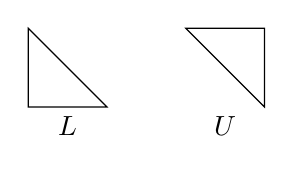
\begin{tikzpicture}
    \draw (0, 0) -- (1, 0) -- (0, 1) -- cycle;
    \node [below] at (0.5, 0) {$L$};
    \begin{scope}[shift={(2, 0)}]
      \draw (1, 1) -- (1, 0) -- (0, 1) -- cycle;
      \node [below] at (0.5, 0) {$U$};
    \end{scope}
  \end{tikzpicture}
\end{center}
Why are triangular matrices nice? First of all, it is easy to find the determinants of triangular matrices. We have
\[
  \det(L) = \prod_{i = 1}^n L_{ii},\quad \det(U) = \prod_{i = 1}^n U_{11}.
\]
In particular, a triangular matrix is non-singular if and only if it has no zero entries in its diagonal.

How do we solve equations involving triangular matrices? Suppose we have a lower triangular matrix equation
\[
  \begin{pmatrix}
    L_{11} & 0 & \cdots & 0\\
    L_{12} & L_{22} & \cdots & 0\\
    \vdots & \vdots & \ddots & \vdots\\
    L_{1n} & L_{2n} & \cdots & L_{nn}
  \end{pmatrix}
  \begin{pmatrix}
    x_1\\
    x_2\\
    \vdots\\
    x_n
  \end{pmatrix}
  =
  \begin{pmatrix}
    b_1\\
    b_2\\
    \vdots\\
    b_n
  \end{pmatrix},
\]
or, more visually, we have
\[
  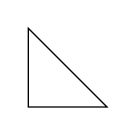
\begin{tikzpicture}[baseline=-0.65ex]
    \draw (0, -0.5) -- (1, -0.5) -- (0, 0.5) -- cycle;
  \end{tikzpicture}
  \;\;
  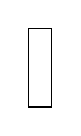
\begin{tikzpicture}[baseline=-0.65ex]
    \draw (0, -0.5) rectangle (0.3, 0.5);
  \end{tikzpicture}
  \;
  =
  \;
  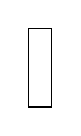
\begin{tikzpicture}[baseline=-0.65ex]
    \draw (0, -0.5) rectangle (0.3, 0.5);
  \end{tikzpicture}
\]
There is nothing to solve in the first line. We can immediately write down the value of $x_1$. Substituting this into the second line, we can then solve for $x_2$. In general, we have
\[
  x_i = \frac{1}{L_{ii}} \left(b_i - \sum_{j = 1}^{i - 1} L_{ij} x_j\right).
\]
This is known as \emph{forward substitution}.

For upper triangular matrices, we can do a similar thing, but we have to solve from the bottom instead. We have
\[
  x_i = \frac{1}{U_{ii}} \left(b_i - \sum_{j = 1 + i}^n U_{ij} x_j\right).
\]
This is known as \emph{backwards substitution}.

This can be used to find the inverse of matrices as well. The solution to $L \mathbf{x}_j = \mathbf{e}_j$ is the $j$th column of $L^{-1}$. It is then easy to see from this that the inverse of a lower triangular matrix is also lower triangular.

Similarly, the columns of $U^{-1}$ are given by solving $U\mathbf{x}_j = \mathbf{e}_i$, and we see that $U^{-1}$ is also upper triangular.

It is helpful to analyse how many operations it takes to compute this. If we look carefully, solving $L\mathbf{x} =\mathbf{b}$ or $U\mathbf{x} = \mathbf{b}$ this way requires $O(n^2)$ operations.

\subsection{LU factorization}
In general, we don't always have triangular matrices. The idea is, for every matrix $A$, find some lower and triangular matrices $L, U$ such that $A = LU$.
\[
  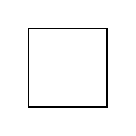
\begin{tikzpicture}[baseline=-0.65ex]
    \draw (0, -0.5) rectangle (1, 0.5);
  \end{tikzpicture}
  \;
  =
  \;
  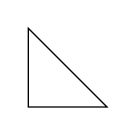
\begin{tikzpicture}[baseline=-0.65ex]
    \draw (0, -0.5) -- (1, -0.5) -- (0, 0.5) -- cycle;
  \end{tikzpicture}
  \;\;
  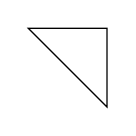
\begin{tikzpicture}[baseline=-0.65ex]
    \draw (1, 0.5) -- (1, -0.5) -- (0, 0.5) -- cycle;
  \end{tikzpicture}
\]
If we can do this, then we can solve $A\mathbf{x} = \mathbf{b}$ in two steps --- we first find a $\mathbf{y}$ such that $L\mathbf{y} = \mathbf{b}$. Then we find an $\mathbf{x}$ such that $U\mathbf{x} = \mathbf{y}$. Then
\[
  A\mathbf{x} = LU\mathbf{x} = L\mathbf{y} = \mathbf{b}.
\]
So what we want is such a factorization. To guarantee uniqueness of the factorization, we require that $L$ is \emph{unit}, i.e.\ the diagonals are all $1$. Otherwise, given any such factorization, we can divide $U$ by some (non-zero) constant and multiply $L$ by the same constant to get another factorization.

\begin{defi}[LU factorization]
  $A = LU$ is an \emph{LU factorization} if $U$ is upper triangular and $L$ is \emph{unit} lower triangular (i.e.\ the diagonals of $L$ are all $1$).
\end{defi}
Note that since $L$ has to be unit, it must be non-singular. However, we still allow $A$ and $U$ to be singular. Note that
\[
  \det (A) = \det (L) \det(U) = \det(U).
\]
So $A$ is singular if and only if $U$ is.

Unfortunately, even if $A$ is non-singular, it may not have an LU factorization. We take a simple example of
\[
  \begin{pmatrix}
    0 & 1\\
    1 & 1
  \end{pmatrix}
\]
This is clearly non-singular, with determinant $-1$. However, we can manually check that there is no LU factorization of this.

On the other hand, while we don't really like singular matrices, singular matrices can still have LU factorizations. For example,
\[
  \begin{pmatrix}
    0 & 0\\
    0 & 1
  \end{pmatrix}
  =
  \begin{pmatrix}
    1 & 0\\
    0 & 1
  \end{pmatrix}
  \begin{pmatrix}
    0 & 0\\
    0 & 1
  \end{pmatrix}
\]
is trivially an LU factorization of a singular matrix.

Fortunately, if $A$ is non-singular and has an LU factorization, then this factorization is unique (this is not necessarily true if $A$ is singular. For example, we know
\[
  \begin{pmatrix}
    0 & 0\\
    0 & 1
  \end{pmatrix}
  =
  \begin{pmatrix}
    1 & 0\\
    a & 1
  \end{pmatrix}
  \begin{pmatrix}
    0 & 0\\
    0 & 1
  \end{pmatrix}
\]
for any real number $a$).

To understand when LU factorizations exist, we try to construct one, and see when it could fail.

We write $L$ in terms of its columns, and $U$ in terms of its rows:
\[
  L =
  \begin{pmatrix}
    \mathbf{l}_1 & \mathbf{l}_2 & \cdots & \mathbf{l}_n
  \end{pmatrix},
  \quad
  U =
  \begin{pmatrix}
    \mathbf{u}_1^T\\
    \mathbf{u}_2^T\\
    \vdots\\
    \mathbf{u}_n^T
  \end{pmatrix}
\]
Clearly, these rows and columns cannot be arbitrary, since $L$ and $U$ are triangular. In particular, $\mathbf{l}_i, \mathbf{u}_i$ must be zero in the first $i - 1$ entries.

Suppose this is an LU factorization of $A$. Then we can write
\[
  A = L\cdot U = \mathbf{l}_1 \mathbf{u}_1^T + \mathbf{l}_2 \mathbf{u}_2^T + \cdots + \mathbf{l}_n \mathbf{u}_n^T.
\]
What do these matrices look like? For each $i$, we know $\mathbf{l}_i$ and $\mathbf{u}_i$ have the first $i - 1$ entries zero. So the first $i - 1$ rows and columns of $\mathbf{l}_i \mathbf{u}_i^T$ are zero. In particular, the first row and columns only have contributions from $\mathbf{l}_1\mathbf{u}_1^T$, the second row/column only has contributions from $\mathbf{l}_2 \mathbf{u}_2^T$ and $\mathbf{l}_1 \mathbf{u}_1^T$ etc.

The plan is as follows:
\begin{enumerate}
  \item Obtain $\mathbf{l}_1$ and $\mathbf{u}_1$ from the first row and column of $A$. Since the first entry of $\mathbf{l}_1$ is $1$, $\mathbf{u}_1^T$ is exactly the first row of $A$. We can then obtain $\mathbf{l}_2$ by taking the first column of $A$ and dividing by $U_{11} = A_{11}$.

  \item Obtain $\mathbf{l}_2$ and $\mathbf{u}_2$ form the second row and column of $A - \mathbf{l}_1 \mathbf{u}_1^T$ similarly.
  \item $\cdots$
  \item Obtain $\mathbf{l}_n$ and $\mathbf{u}_n^T$ from the $n$th row and column of $A - \sum_{i = 1}^{n - 1} \mathbf{l}_i \mathbf{u}_i^T$.
\end{enumerate}
We can turn this into an algorithm. We define the intermediate matrices, starting with
\[
  A^{(0)} = A.
\]
For $k = 1, \cdots, n$, we let
\begin{align*}
  U_{kj} &= A_{kj}^{(k - 1)} & j &=k, \cdots, n\\
  L_{ik} &= \frac{A_{ik}}{A_{kk}^{(k - 1)}} & i &= k, \cdots, n\\
  A_{ij}^{(k)} &= A_{ij}^{(k - 1)} - L_{ik} U_{kj} & i, j &\geq k
\end{align*}
When $k = n$, we end up with a zero matrix, and then $U$ and $L$ are completely filled.

We can now see when this will break down. A sufficient condition for $A = LU$ to exist is that $A_{kk}^{(k - 1)} \not= 0$ for all $k$. Since $A_{kk}^{(k - 1)} = U_{kk}$, this sufficient condition ensures $U$, and hence $A$ is non-singular. Conversely, if $A$ is non-singular and an LU factorization exists, then this would always work, since we must have $A_{kk}^{(k - 1)} = U_{kk} \not= 0$. Moreover, the LU factorization must be given by this algorithm. So we get uniqueness.

The problem with this sufficient condition is that most of these coefficients do not appear in the matrix $A$. They are constructed during the algorithm. We don't know easily what they are in terms of the coefficients of $A$. We will later come up with an equivalent condition on our original $A$ that is easier to check.

Note that as long as this method does not break down, we need $O(n^3)$ operations to perform this factorization. Recall we only needed $O(n^2)$ operations to solve the equation after factorization. So the bulk of the work in solving $A\mathbf{x} = \mathbf{b}$ is in doing the LU factorization.

As before, this allows us to find the inverse of $A$ if it is non-singular. In particular, solving $A\mathbf{x}_j = \mathbf{e}_j$ gives the $j$th column of $A^{-1}$. Note that we are solving the system for the same $A$ for each $j$. So we only have to perform the LU factorization once, and then solve $n$ different equations. So in total we need $O(n^3)$ operations.

However, we still have the problem that factorization is not always possible. Requiring that we must factorize $A$ as $LU$ is too restrictive. The idea is to factor something closely related, but not exactly $A$. Instead, we want a factorization
\[
  PA = LU,
\]
where $P$ is a permutation matrix. Recall a permutation matrix acting on a column vector just permutes the elements of the vector, and $P$ acting on $A$ would just permute the rows of $A$. So we want to factor $A$ up to a permutation of rows.

Our goal now is to extend the previous algorithm to allow permutations of rows, and then we shall show that we will be able to perform this factorization all the time.

Suppose our breakdown occurs at $k = 1$, i.e.\ $A_{11}^{(0)} = A_{11} = 0$. We find a permutation matrix $P_1$ and let it act via $P_1A^{(0)}$. The idea is to look down the first column of $A$, and find a row starting with a non-zero element, say $p$. Then we use $P_1$ to interchange rows $1$ and $p$ such that $P_1A^{(0)}$ has a non-zero top-most entry. For simplicity, we assume we always need a $P_1$, and if $A_{11}^{(0)}$ is non-zero in the first place, we just take $P_1$ to be the identity.

After that, we can carry on. We construct $\mathbf{l}_1$ and $\mathbf{u}_1$ from $P_1A^{(0)}$ as before, and set $A^{(1)} = P_1A^{(0)} - \mathbf{l}_1 \mathbf{u}_1^T$.

But what happens if the first column of $A$ is completely zero? Then no interchange will make the $(1, 1)$ entry non-zero. However, in this case, we don't actually have to do anything. We can immediately find our $\mathbf{l}_1$ and $\mathbf{u}_1$, namely set $\mathbf{l}_1 = \mathbf{e}_1$ (or anything) and let $\mathbf{u}_1^T$ be the first row of $A^{(0)}$. Then this already works. Note however that this corresponds to $A$ (and hence $U$) being singular, and we are not too interested with these.

The later steps are exactly analogous. Suppose we have $A_{kk}^{(k - 1)} = 0$. Again we find a $P_k$ such that $P_k A^{(k - 1)}$ has a non-zero $(k, k)$ entry. We then construct $\mathbf{l}_k$ and $\mathbf{u}_k$ from $P_k A^{(k - 1)}$ and set
\[
  A^{(k)} = P_k A^{(n - 1)} - \mathbf{l}_k \mathbf{u}_k^t.
\]
Again, if the $k$th column of $A^{(k - 1)}$ is completely zero, we set $\mathbf{l}_k = \mathbf{e}_k$ and $\mathbf{u}_k^T$ to be the $k$th row of $A^{(k - 1)}$. But again this implies $A$ and $U$ will be singular.

However, as we do this, the permutation matrices appear all over the place inside the algorithm. It is not immediately clear that we do get a factorization of the form $PA = LU$. Fortunately, keeping track of the interchanges, we \emph{do} have an LU factorization
\[
  PA = \tilde{L}U,
\]
where $U$ is what we got from the algorithm,
\[
  P = P_{n - 1} \cdots P_2 P_1,
\]
while $\tilde{L}$ is given by
\[
  \tilde{L} =
  \begin{pmatrix}
    \tilde{\mathbf{l}}_1 & \cdots & \tilde{\mathbf{l}}_n
  \end{pmatrix},
  \quad \tilde{\mathbf{l}}_k = P_{n - 1} \cdots P_{k - 1} \mathbf{l}_k.
\]
Note that in particular, we have
\[
  \tilde{\mathbf{l}}_{n - 1} = \mathbf{l}_{n - 1},\quad \tilde{\mathbf{l}}_n = \mathbf{l}_n.
\]
One problem we have not considered is the problem of inexact arithmetic. While these formula are correct mathematically, when we actually implement things, we do them on computers with finite precision. As we go through the algorithm, errors will accumulate, and the error might be amplified to a significant amount when we get the reach the end. We want an algorithm that is insensitive to errors. In order to work safely in inexact arithmetic, we will put the element of \emph{largest} modulus in the $(k, k)$th position, not just an arbitrary non-zero one, as this minimizes the error when dividing.

\subsection{\texorpdfstring{$A = LU$}{A = LU} for special \texorpdfstring{$A$}{A}}
There is one thing we haven't figured out yet. Can we just look at the matrix $A$, and then determine whether it has an LU factorization (that does not involve permutations)? To answer this, we start with some definitions.

\begin{defi}[Leading principal submatrix]
  The \emph{leading principal submatrices} $A_k \in \R^{k \times k}$ for $k = 1, \cdots, n$ of $A \in \R^{n \times n}$ are
  \[
    (A_k)_{ij} = A_{ij},\quad i, j = 1, \cdots, k.
  \]
  In other words, we take the first $k$ rows and columns of $A$.
\end{defi}

\begin{thm}
  A sufficient condition for the existence for both the existence and uniqueness of $A = LU$ is that $\det(A_{k}) \not= 0$ for $k = 1, \cdots, n - 1$.
\end{thm}
Note that we don't need $A$ to be non-singular. This is equivalent to the restriction $A_{kk}^{(k - 1)} \not= 0$ for $k = 1, \cdots, n - 1$. Also, this is a \emph{sufficient} condition, not a necessary one.

\begin{proof}
  Straightforward induction. % include
\end{proof}

We extend this result a bit:
\begin{thm}
  If $\det (A_k) \not= 0$ for all $k = 1, \cdots, n$, then $A \in R^{n \times n}$ has a unique factorization of the form
  \[
    A = LD \hat{U},
  \]
  where $D$ is non-singular diagonal matrix, and both $L$ and $\hat{U}$ are unit triangular.
\end{thm}

\begin{proof}
  From the previous theorem, $A = LU$ exists. Since $A$ is non-singular, $U$ is non-singular. So we can write this as
  \[
    U = D\hat{U},
  \]
  where $D$ consists of the diagonals of $U$ and $\hat{U} = D^{-1}U$ is unit.
\end{proof}
This is not hard, but is rather convenient. In particular, it allows us to factorize symmetric matrices in a nice way.

\begin{thm}
  Let $A \in \R^{n \times n}$ be non-singular and $\det(A_k) \not= 0$ for all $k = 1, \cdots, n$. Then there is a unique ``symmetric'' factorization
  \[
    A = LDL^T,
  \]
  with $L$ unit lower triangular and $D$ diagonal and non-singular.
\end{thm}

\begin{proof}
  From the previous theorem, we can factorize $A$ uniquely as
  \[
    A = LD\hat{U}.
  \]
  We take the transpose to obtain
  \[
    A = A^T = \hat{U}^T D L^T.
  \]
  This is a factorization of the form ``unit lower''-``diagonal''-``unit upper''. By uniqueness, we must have $\hat{U} = L^T$. So done.
\end{proof}

We just looked at a special type of matrices, the symmetric matrices. We look at another type of matrices:
\begin{defi}[Positive definite matrix]
  A matrix $A \in R^{n\times n}$ is \emph{positive-definite} if
  \[
    \mathbf{x}^T A\mathbf{x} > 0
  \]
  for $\mathbf{x}\not= \mathbf{0} \in \R^n$.
\end{defi}

\begin{thm}
  Let $A \in \R^{n\times n}$ be a positive-definite matrix. Then $\det(A_k) \not= 0$ for all $k = 1, \cdots, n$.
\end{thm}

\begin{proof}
  First consider $k = n$. To show $A$ is non-singular, it suffices to show that $A\mathbf{x} = \mathbf{0}$ implies $\mathbf{x} = \mathbf{0}$. But we can multiply the equation by $\mathbf{x}^T$ to obtain $\mathbf{x}^T A\mathbf{x} = 0$. By positive-definiteness, we must have $\mathbf{x} = \mathbf{0}$. So done.

  Now suppose $A_k \mathbf{y} = \mathbf{0}$ for $k < n$ and $\mathbf{y} = \R^k$. Then $\mathbf{y}^T A_k \mathbf{y} = 0$. We invent a new $\mathbf{x} \in \R^n$ by taking $\mathbf{y}$ and pad it with zeros. Then $\mathbf{x}^T A\mathbf{x} = 0$. By positive-definiteness, we know $\mathbf{x} = \mathbf{0}$. Then in particular $\mathbf{y} = \mathbf{0}$.
\end{proof}

We are going to use this to prove the most important result in this section. We are going to consider matrices that are symmetric \emph{and} positive-definite.

\begin{thm}
  A symmetric matrix $A \in \R^{n \times n}$ is \emph{positive-definite} iff we can factor it as
  \[
    A = LDL^T,
  \]
  where $L$ is unit lower triangular, $D$ is diagonal and $D_{kk} > 0$.
\end{thm}

\begin{proof}
  First suppose such a factorization exists, then
  \[
    \mathbf{x}^T A\mathbf{x} = \mathbf{x}^T L DL^T \mathbf{x} = (L^T\mathbf{x})^T D(L^T\mathbf{x}).
  \]
  We let $\mathbf{y} = L^T\mathbf{x}$. Note that $\mathbf{y} = \mathbf{0}$ if and only if $\mathbf{x} = \mathbf{0}$, since $L$ is invertible. So
  \[
    \mathbf{x}^TA\mathbf{x} = \mathbf{y}^T D\mathbf{y} = \sum_{k = 1}^n y_k^2 D_{kk} > 0
  \]
  if $\mathbf{y} \not= 0$.

  Now if $A$ is positive definite, it has an LU factorization, and since $A$ is symmetric, we can write it as
  \[
    A = LDL^T,
  \]
  where $L$ is unit lower triangular and $D$ is diagonal. Now we have to show $D_{kk} > 0$. We define $\mathbf{y}_k$ such that $L^T \mathbf{y}_k = \mathbf{e}_k$, which exist, since $L$ is invertible. Then clearly $\mathbf{y}_k \not= \mathbf{0}$. Then we have
  \[
    D_{kk} = \mathbf{e}_k^T D\mathbf{e}_k = \mathbf{y}_k^T LDL^T \mathbf{y}_k = \mathbf{y}_k^T A\mathbf{y}_k > 0.
  \]
  So done.
\end{proof}
This is a practical check for symmetric $A$ being positive definite. We can perform this LU factorization, and then check whether the diagonal has positive entries.

\begin{defi}[Cholesky factorization]
  The \emph{Cholesky factorization} of a symmetric positive-definite matrix $A$ is a factorization of the form
  \[
    A = LDL^T,
  \]
  with $L$ unit lower triangular and $D$ a positive-definite diagonal matrix.
\end{defi}
There is another way of doing this. We let $D^{1/2}$ be the ``square root'' of $D$, by taking the positive square root of the diagonal entries of $D$. Then we have
\[
  A = LDL^T = LD^{1/2}D^{1/2}L^T = (LD^{1/2})(LD^{1/2})^T = GG^T,
\]
where $G$ is lower triangular with $G_{kk} > 0$. This is another way of presenting this result.

Finally, we look at the LU factorization of band matrices.
\begin{defi}[Band matrix]
  A \emph{band matrix} of \emph{band width} $r$ is a matrix $A$ such that $A_{ij} \not= 0$ implies $|i - j| \leq r$.
\end{defi}
For example, a band matrix of band width $0$ is a diagonal matrix; a band matrix of band width $1$ is a tridiagonal matrix.
\begin{center}
  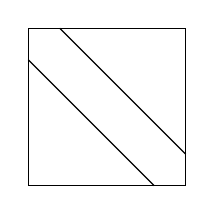
\begin{tikzpicture}
    \draw (0, 0) rectangle (2, 2);
    \draw (0, 1.6) -- (1.6, 0);
    \draw (0.4, 2) -- (2, 0.4);
  \end{tikzpicture}
\end{center}
The result is
\begin{prop}
  If a band matrix $A$ has band width $r$ and an LU factorization $A = LU$, then $L$ and $U$ are both band matrices of width $r$.
\end{prop}

\begin{proof}
  Straightforward verification.
\end{proof}

\section{Linear least squares}
Finally, we consider a slightly different kind of problem, whose solution involves a different kind of factorization.

The question we are interested in is how we can ``solve''
\[
  A\mathbf{x} = \mathbf{b},
\]
where $A \in \R^{m \times n}$, with $m > n$, and $\mathbf{b} \in \R^m$ and $\mathbf{x} \in \R^n$.

Of course, this is an over-determined system. In general, this has no solution. So we want to find the ``best'' solution to this system of equations. More precisely, we want to find an $\mathbf{x}^* \in \R^n$ that minimizes $\|A\mathbf{x} - \mathbf{b}\|^2$. Note that we use the Euclidean norm. This is the \emph{least squares problem}.

Why would one be interested in this? Often in, say, statistics, we have some linear model that says the outcome $B$ is related to the input variables $A_1, \cdots, A_n$ by
\[
  B = A_1 X_1 + A_2 X_2 + \cdots + A_n X_n + \varepsilon,
\]
where the $X_i$ are some unknown parameters, and $\varepsilon$ is some random fluctuation. The idea is to do lots of experiments, say $m$ of them, collect the data in $A \in R^{m \times n}$ and $\mathbf{b} \in R^m$, and then find the $X_i$'s that predict these results the most accurately, i.e.\ find the $\mathbf{x}$ such that $A\mathbf{x}$ is as close to $\mathbf{b}$ as possible.

So how can we find this $\mathbf{x}^*$? First of all, we find a necessary and sufficient condition for $\mathbf{x}^*$ to be a solution to this.
\begin{thm}
  A vector $\mathbf{x}^* \in \R^n$ minimizes $\|A\mathbf{x} - \mathbf{b}\|^2$ if and only if
  \[
    A^T(A\mathbf{x}^* - \mathbf{b}) = 0.
  \]
\end{thm}

\begin{proof}
  A solution, by definition, minimizes
  \begin{align*}
    f(\mathbf{x}) &= \bra A\mathbf{x} - \mathbf{b}, A\mathbf{x} - \mathbf{b}\ket\\
    &= \mathbf{x}^T AA\mathbf{x} - 2\mathbf{x}^T A^T \mathbf{b} + \mathbf{b}^T \mathbf{b}.
  \end{align*}
  Then as a function of $\mathbf{x}$, the partial derivatives of this must vanish. We have
  \[
    \nabla f(\mathbf{x}) = 2A^T(A\mathbf{x} - \mathbf{b}).
  \]
  So a necessary condition is
  \[
    A^T (A\mathbf{x} - \mathbf{b}).
  \]
  Now suppose our $\mathbf{x}^*$ satisfies $A^T (A\mathbf{x}^* - \mathbf{b}) = 0$. Then for all $\mathbf{x} \in \R^n$, we write $\mathbf{x} = \mathbf{x}^* + \mathbf{y}$, and then we have
  \begin{align*}
    \|A\mathbf{x} - \mathbf{b}\|^2 &= \|A(\mathbf{x}^* + \mathbf{y}) - \mathbf{b}\|\\
    &= \|A \mathbf{x}^* - \mathbf{b}\| + 2\mathbf{y}^T A^T (A\mathbf{x} - \mathbf{b}) + \|A\mathbf{y}\|^2\\
    &= \|A \mathbf{x}^* - \mathbf{b}\| + \|A\mathbf{y}\|^2\\
    &\geq \|A \mathbf{x}^* - \mathbf{b}\|.
  \end{align*}
  So $\mathbf{x}^*$ must minimize the Euclidean norm.
\end{proof}

\begin{cor}
  If $A \in \R^{m \times n}$ is a full-rank matrix, then there is a unique solution to the least squares problem.
\end{cor}

\begin{proof}
  We know all minimizers are solutions to
  \[
    (A^T A)\mathbf{x} = A^T \mathbf{b}.
  \]
  The matrix $A$ being full rank means $\mathbf{y} \not= \mathbf{0} \in \R^n$ implies $A\mathbf{y} \not= \mathbf{0} \in \R^m$. Hence $A^T A \in \R^{n \times n}$ is positive definite (and in particular non-singular), since
  \[
    \mathbf{x}^TA^T A\mathbf{x} = (A \mathbf{x})^T (A \mathbf{x}) = \|A \mathbf{x}\|^2 > 0
  \]
  for $\mathbf{x} \not= \mathbf{0}$. So we can invert $A^T A$ and find a unique solution $\mathbf{x}$.
\end{proof}

Now to find the minimizing $\mathbf{x}^*$, we need to solve the \emph{normal equations}
\[
  A^T A\mathbf{x} = A^T \mathbf{b}.
\]
If $A$ has full rank, then $A^T A$ is non-singular, and there is a unique solution. If not, then the general theory of linear equations tells us there are either infinitely many solution or no solutions. But for this particular form of equations, it turns out we can show this is always consistent. So there will always be a solution. However, solving these equations is not the recommended algorithm for finding $\mathbf{x}^*$ for accuracy reasons. Instead the solution of these is based on orthogonal matrices.

\begin{defi}[Orthogonal matrix]
  A square matrix $Q \in \R^{n \times n}$ is orthogonal if $Q^T Q = I$.
\end{defi}

A key property of the orthogonal matrices is that we have
\[
  \|Q\mathbf{x}\| = \|\mathbf{x}\|
\]
for all $\mathbf{x} \in \R^n$. This is helpful since what we are trying to do in the least-squares problem involves minimizing the Euclidean norm of something.

The idea is that for any orthogonal matrix, minimizing $\|A\mathbf{x} - \mathbf{b}\|$ is the same as minimizing $\|QA \mathbf{x} - Q\mathbf{b}\|$. So $Q$ should we pick? Recall that a simple kind of matrices is triangular matrices. So we might want to get something, say, upper triangular.

\begin{defi}[QR factorization]
  A \emph{QR factorization} of an $m \times n$ matrix $A$ is a factorization of the form
  \[
    A = QR,
  \]
  where $Q \in \R^{m \times m}$ is an orthogonal matrix, and $R \in \R^{m \times n}$ is ``upper triangular'' matrix, where ``upper triangular'' means
  \[
    R =
    \begin{pmatrix}
      R_{11} & R_{12} & \cdots & R_{1m}\\
      0 & R_{22} & \cdots & R_{2m}\\
      \vdots & \vdots & \ddots & \vdots\\
      0 & 0 & \cdots & R_{mm}\\
      0 & 0 & \cdots & 0\\
      \vdots & \vdots & \ddots & \vdots\\
      0 & 0 & \cdots & 0
    \end{pmatrix}
  \]
\end{defi}
Note that every $A \in R^{m \times n}$ has a QR factorization, as we will soon show, but this is not unique (e.g.\ we can multiply both $Q$ and $R$ by $-1$).

Once we have the QR factorization, we can multiply $\|A\mathbf{x} - \mathbf{b}\|$ by $Q^T = Q^{-1}$, and get an equivalent problem of minimizing $\|R \mathbf{x} - Q^T \mathbf{b}\|$. We will not go into details, but it should be clear that this is not too hard to solve.

There is an alternative ``skinny'' QR factorization, with $A = \tilde{Q} \tilde{R}$, where we remove redundant rows and columns such that $\tilde{Q} \in \R^{m \times n}$ and $\tilde{R} \in \R^{n \times n}$. % insert some pictures.
This is good enough to solve the least squares problem.

We will see that if $A$ has full rank, then the skinny QR is unique up to a sign, i.e.\ if we require $\tilde{R}_{kk} > 0$ for $k = 1, \cdots, n$.

We shall demonstrate three standard algorithms for QR factorization:
\begin{enumerate}
  \item Gram-Schmidt factorization
  \item Givens rotations
  \item Householder reflections
\end{enumerate}
The latter two are based on some geometric ideas, while the first is based on the familiar Gram-Schmidt process.

\subsubsection*{Gram-Schmidt factorization}
This targets the skinny version. So we stop writing the tildes above, and just write $Q \in \R^{m \times n}$ and $R \in \R^{n \times n}$.

As we all know, the Gram-Schmidt process orthogonalizes vectors. What we are going to orthogonalize are the columns of $A$. We write
\[
  A =
  \begin{pmatrix}
    \mathbf{a}_1 & \cdots & \mathbf{a}_n
  \end{pmatrix},\quad
  Q =
  \begin{pmatrix}
    \mathbf{q}_1 & \cdots & \mathbf{q}_n
  \end{pmatrix}.
\]
By definition of the QR factorization, we need
\[
  \mathbf{a}_j = \sum_{i = 1}^j R_{ij} \mathbf{q}_i.
\]
This is just done in the usual Gram-Schmidt way.
\begin{enumerate}
  \item To construct column $1$, if $\mathbf{a}_1 \not= \mathbf{0}$, then we set
    \[
      \mathbf{q}_1 = \frac{\mathbf{a}_1}{\|\mathbf{a}_1\|},\quad R_{11} = \|\mathbf{a}_1\|.
    \]
    Note that the only non-unique possibility here is the sign --- we can let $R_{11} = - \|\mathbf{a}_1\|$ and $\mathbf{q}_1 = -\frac{\mathbf{a}_1}{\|\mathbf{a}_1\|}$ instead. But if we require $R_{11} > 0$, then this is fixed.

    In the degenerate case, $\mathbf{a}_1 = \mathbf{0}$, then we can just set $R_{11} = 0$, and the pick any $\mathbf{q}_1 \in \R^n$ with $\|\mathbf{q}_1\| = 1$.
  \item For columns $1 < k \leq n$, for $i = 1, \cdots, k - 1$, we set
    \[
      R_{ik} = \bra \mathbf{q}_i, \mathbf{a}_k\ket,
    \]
    and set
    \[
      \mathbf{d}_k = \mathbf{a}_k - \sum_{i = 1}^{k - 1} \mathbf{q}_i \bra \mathbf{q}_i, \mathbf{a}_k\ket.
    \]
    If $\mathbf{d}_k \not= \mathbf{0}$, then we set
    \[
      \mathbf{q}_k = \frac{\mathbf{d}_k}{\|\mathbf{d}_k\|},
    \]
    and
    \[
      R_{kk} = \|\mathbf{d}_k\|.
    \]
    In the case where $\mathbf{d}_k = \mathbf{0}$, we again set $R_{kk} = 0$, and pick $\mathbf{q}_k$ to be anything orthonormal to $\mathbf{q}_1, \cdots, \mathbf{q}_{k - 1}$.
\end{enumerate}

In practice, a slightly different algorithm (modified Gram-Schmidt process) is used, which is (much) superior with inexact arithmetic. The modified Gram-Schmidt process is in fact the same algorithm, but performed in a different order in order to minimize errors.

However, this is often not an ideal algorithm for large matrices, since there are many divisions and normalizations involved in computing the $\mathbf{q}_i$, and the accumulation of errors will cause the resulting matrix $Q$ to lose orthogonality.

\subsubsection*{Givens rotations}
This works with the full QR factorization.

Recall that in $\R^2$, a clockwise rotation of $\theta \in [-\pi, \pi]$ is performed by
\[
  \begin{pmatrix}
    \cos \theta & \sin \theta\\
    -\sin \theta & \cos \theta
  \end{pmatrix}
  \begin{pmatrix}
    \alpha\\ \beta
  \end{pmatrix}
  =
  \begin{pmatrix}
    \alpha \cos \theta + \beta \sin \theta\\
    -\alpha \sin \theta + \beta \cos \theta
  \end{pmatrix}.
\]
By choosing $\theta$ such that
\[
  \cos \theta = \frac{\alpha}{\sqrt{\alpha^2 + \beta^2}},\quad \sin \theta = \frac{\beta}{\sqrt{\alpha^2 + \beta^2}},
\]
this then becomes
\[
  \begin{pmatrix}
    \sqrt{\alpha^2 + \beta^2}\\
    0
  \end{pmatrix}.
\]
Of course, by choosing a slightly different $\theta$, we can make the result zero in the first component and $\sqrt{\alpha^2 + \beta^2}$ in the second.

\begin{defi}[Givens rotation]
  In $\R^m$, where $m > 2$, we define the \emph{Givens rotation} on $3$ parameters $1 \leq p < q \leq m, \theta \in [-\pi, \pi]$ by
  \setcounter{MaxMatrixCols}{11}
  \[
    \Omega_\theta^{[p, q]} =
    \begin{pmatrix}
      1 &\\
      & \ddots\\
      & & 1\\
      & & & \cos \theta & & & & \sin \theta\\
      & & & & 1\\
      & & & & & \ddots\\
      & & & & & & 1\\
      & & & -\sin \theta & & & & \cos \theta\\
      & & & & & & & & 1\\
      & & & & & & & & & \ddots\\
      & & & & & & & & & & 1
    \end{pmatrix} \in \R^{m \times m},
  \]
  where the $\sin$ and $\cos$ appear at the $p, q$th rows and columns.
\end{defi}
Note that for $\mathbf{y} \in \R^m$, the effect of $\Omega_\theta^{[p, q]}$ only alters the $p$ and $q$ components. In general, for $B \in \R^{m \times n}$, then $\Omega_\theta^{[p, q]} B$ only alters the $p$ and $q$ rows of $B$.

Moreover, just like the $\R^2$ case, given a particular $\mathbf{z} \in \R^m$, we can choose $\theta$ such that the $q$th component $(\Omega^{[p, q]}_\theta \mathbf{z})_q = 0$.

Hence, $A \in \R^{m \times n}$ can be transformed into an ``upper triangular'' form by applying $s = mn - \frac{n(n + 1)}{2}$ Givens rotations, since we need to introduce $s$ many zeros. Then
\[
  Q_s \cdots Q_1 A = R.
\]
How exactly do we do this? Instead of writing down a general algorithm, we illustrate it with a matrix $A \in R^{4 \times 3}$. The resultant $R$ would look like
\[
  R =
  \begin{pmatrix}
    R_{11} & R_{12} & R_{13}\\
    0 & R_{22} & R_{23}\\
    0 & 0 & R_{33}\\
    0 & 0 & 0
  \end{pmatrix}.
\]
We will apply the Givens rotations in the following order:
\[
  \Omega_{\theta_6}^{[3, 4]}\Omega_{\theta_5}^{[3, 4]} \Omega_{\theta_4}^{[2, 3]} \Omega_{\theta_3}^{[1, 4]} \Omega_{\theta_2}^{[1, 3]} \Omega_{\theta_1}^{[1, 2]} A = R.
\]
The matrix $A$ transforms as follows:
\begin{center}
  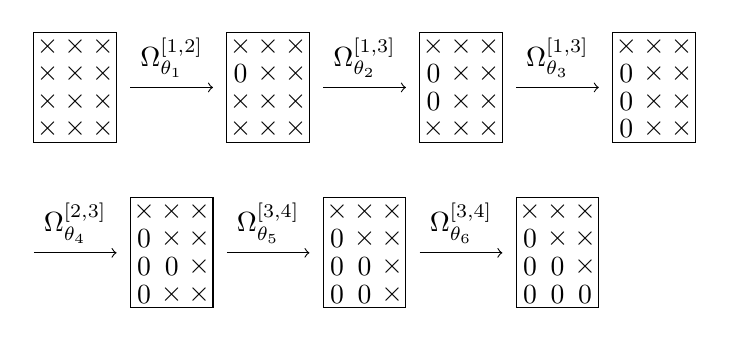
\begin{tikzpicture}[scale=0.35]
    \begin{scope}
      \draw (-1.5, -2) rectangle (1.5, 2);
      \node at (-1, 1.5) {$\times$}; \node at (0, 1.5) {$\times$}; \node at (1, 1.5) {$\times$};
      \node at (-1, 0.5) {$\times$}; \node at (0, 0.5) {$\times$}; \node at (1, 0.5) {$\times$};
      \node at (-1, -0.5) {$\times$}; \node at (0, -0.5) {$\times$}; \node at (1, -0.5) {$\times$};
      \node at (-1, -1.5) {$\times$}; \node at (0, -1.5) {$\times$}; \node at (1, -1.5) {$\times$};
      \draw [->] (2, 0) -- (5, 0) node [pos=0.5, above] {$\Omega_{\theta_1}^{[1, 2]}$};
    \end{scope}

    \begin{scope}[shift={(7, 0)}]
      \draw (-1.5, -2) rectangle (1.5, 2);
      \node at (-1, 1.5) {$\times$}; \node at (0, 1.5) {$\times$}; \node at (1, 1.5) {$\times$};
      \node at (-1, 0.5) {$0$}; \node at (0, 0.5) {$\times$}; \node at (1, 0.5) {$\times$};
      \node at (-1, -0.5) {$\times$}; \node at (0, -0.5) {$\times$}; \node at (1, -0.5) {$\times$};
      \node at (-1, -1.5) {$\times$}; \node at (0, -1.5) {$\times$}; \node at (1, -1.5) {$\times$};
      \draw [->] (2, 0) -- (5, 0) node [pos=0.5, above] {$\Omega_{\theta_2}^{[1, 3]}$};
    \end{scope}
    \begin{scope}[shift={(14, 0)}]
      \draw (-1.5, -2) rectangle (1.5, 2);
      \node at (-1, 1.5) {$\times$}; \node at (0, 1.5) {$\times$}; \node at (1, 1.5) {$\times$};
      \node at (-1, 0.5) {$0$}; \node at (0, 0.5) {$\times$}; \node at (1, 0.5) {$\times$};
      \node at (-1, -0.5) {$0$}; \node at (0, -0.5) {$\times$}; \node at (1, -0.5) {$\times$};
      \node at (-1, -1.5) {$\times$}; \node at (0, -1.5) {$\times$}; \node at (1, -1.5) {$\times$};
      \draw [->] (2, 0) -- (5, 0) node [pos=0.5, above] {$\Omega_{\theta_3}^{[1, 3]}$};
    \end{scope}

    \begin{scope}[shift={(21, 0)}]
      \draw (-1.5, -2) rectangle (1.5, 2);
      \node at (-1, 1.5) {$\times$}; \node at (0, 1.5) {$\times$}; \node at (1, 1.5) {$\times$};
      \node at (-1, 0.5) {$0$}; \node at (0, 0.5) {$\times$}; \node at (1, 0.5) {$\times$};
      \node at (-1, -0.5) {$0$}; \node at (0, -0.5) {$\times$}; \node at (1, -0.5) {$\times$};
      \node at (-1, -1.5) {$0$}; \node at (0, -1.5) {$\times$}; \node at (1, -1.5) {$\times$};
    \end{scope}

    \begin{scope}[shift={(3.5, -6)}]
      \draw [->] (-5, 0) -- (-2, 0) node [pos=0.5, above] {$\Omega_{\theta_4}^{[2, 3]}$};
      \draw (-1.5, -2) rectangle (1.5, 2);
      \node at (-1, 1.5) {$\times$}; \node at (0, 1.5) {$\times$}; \node at (1, 1.5) {$\times$};
      \node at (-1, 0.5) {$0$}; \node at (0, 0.5) {$\times$}; \node at (1, 0.5) {$\times$};
      \node at (-1, -0.5) {$0$}; \node at (0, -0.5) {$0$}; \node at (1, -0.5) {$\times$};
      \node at (-1, -1.5) {$0$}; \node at (0, -1.5) {$\times$}; \node at (1, -1.5) {$\times$};
      \draw [->] (2, 0) -- (5, 0) node [pos=0.5, above] {$\Omega_{\theta_5}^{[3, 4]}$};
    \end{scope}

    \begin{scope}[shift={(10.5, -6)}]
      \draw (-1.5, -2) rectangle (1.5, 2);
      \node at (-1, 1.5) {$\times$}; \node at (0, 1.5) {$\times$}; \node at (1, 1.5) {$\times$};
      \node at (-1, 0.5) {$0$}; \node at (0, 0.5) {$\times$}; \node at (1, 0.5) {$\times$};
      \node at (-1, -0.5) {$0$}; \node at (0, -0.5) {$0$}; \node at (1, -0.5) {$\times$};
      \node at (-1, -1.5) {$0$}; \node at (0, -1.5) {$0$}; \node at (1, -1.5) {$\times$};
      \draw [->] (2, 0) -- (5, 0) node [pos=0.5, above] {$\Omega_{\theta_6}^{[3, 4]}$};
    \end{scope}

    \begin{scope}[shift={(17.5, -6)}]
      \draw (-1.5, -2) rectangle (1.5, 2);
      \node at (-1, 1.5) {$\times$}; \node at (0, 1.5) {$\times$}; \node at (1, 1.5) {$\times$};
      \node at (-1, 0.5) {$0$}; \node at (0, 0.5) {$\times$}; \node at (1, 0.5) {$\times$};
      \node at (-1, -0.5) {$0$}; \node at (0, -0.5) {$0$}; \node at (1, -0.5) {$\times$};
      \node at (-1, -1.5) {$0$}; \node at (0, -1.5) {$0$}; \node at (1, -1.5) {$0$};
    \end{scope}
  \end{tikzpicture}
\end{center}
Note that when applying, say, $\Omega_{\theta_4}^{[2, 3]}$, the zeros of the first column get preserved, since $\Omega_{\theta_4}^{[2, 3]}$ only mixes together things in row $2$ and $3$, both of which are zero in the first column. So we are safe.

Note that this gives us something of the form
\[
  Q_s \cdots Q_1 A = R.
\]
We can obtain a QR factorization by inverting to get
\[
  A = Q_1^T \cdots Q_s^T R.
\]
However, we don't really need to do this if we just want to do use this to solve the least squares problem, since to do so, we need to multiply by $Q^T$, not $Q$, which is exactly $Q_s \cdots Q_1$.

\subsubsection*{Householder reflections}
\begin{defi}[Householder reflection]
  For $\mathbf{u} \not= \mathbf{0} \in \R^m$, we define the \emph{Householder reflection} by
  \[
    H_{\mathbf{u}} = I - 2\frac{\mathbf{u}\mathbf{u}^T}{ \mathbf{u}^T \mathbf{u}} \in \R^{m \times m}.
  \]
\end{defi}
Note that this is symmetric, and we can see $H_{\mathbf{u}}^2 = I$. So this is indeed orthogonal.

To show this is a reflection, suppose we resolve $\mathbf{x}$ as the perpendicular and parallel parts as $\mathbf{x} = \alpha \mathbf{u} + \mathbf{w} \in \R^m$, where
\[
  \alpha = \frac{\mathbf{u}^T \mathbf{x}}{\mathbf{u}^T \mathbf{u}},\quad \mathbf{u}^T \mathbf{w} = 0.
\]
Then we have
\[
  H_{\mathbf{u}} \mathbf{x} = -\alpha \mathbf{u} + \mathbf{w}.
\]
So this is a reflection in the $m - 1$-dimensional hyperplane $\mathbf{u}^T \mathbf{y} = 0$.

What is the cost of computing $H_{\mathbf{u}}\mathbf{z}$? This is evaluated as
\[
  H_{\mathbf{u}}\mathbf{z} = \mathbf{z} - 2\frac{\mathbf{u}^T \mathbf{z}}{\mathbf{u}^T \mathbf{u}}\mathbf{u}.
\]
This only requires $O(m)$ operations, which is nice.

\begin{prop}
  A matrix $A \in \R^{m \times n}$ can be transformed into upper-triangular form by applying $n$ Householder reflections, namely
  \[
    H_n \cdots H_1 A = R,
  \]
  where each $H_n$ introduces zero into column $k$ and leaves the other zeroes alone.
\end{prop}
This is much less multiplications needed than the number needed for Givens rotations, in general.

To show this, we first prove some lemmas.

\begin{lemma}
  Let $\mathbf{a}, \mathbf{b} \in \R^m$, with $\mathbf{a} \not= \mathbf{b}$, but $\|\mathbf{a}\| = \|\mathbf{b}\|$. Then if we pick $\mathbf{u} = \mathbf{a} - \mathbf{b}$, then
  \[
    H_\mathbf{u} \mathbf{a} = \mathbf{b}.
  \]
\end{lemma}
This is obvious if we draw some pictures in low dimensions.
\begin{proof}
  We just do it:
  \[
    H_\mathbf{u} \mathbf{a} = \mathbf{a} - \frac{2(\|\mathbf{a}\| - \mathbf{a}^T \mathbf{b})}{\|\mathbf{a}\|^2 - 2\mathbf{a}^T \mathbf{b} + \|\mathbf{b}\|^2} (\mathbf{a} - \mathbf{b}) = \mathbf{a} - (\mathbf{a} - \mathbf{b}) = \mathbf{b},
  \]
  where we used the fact that $\|\mathbf{a}\| = \|\mathbf{b}\|$.
\end{proof}
We will keep applying the lemma. Since we want to get an upper triangular matrix, it makes sense to pick $\mathbf{b}$ to have many zeroes, and the best option would be to pick $\mathbf{b}$ to be a unit vector.

So we begin our algorithm: we want to clear the first column of $A$. We let $\mathbf{a}$ be the first column of $A$, and assume $\mathbf{a} \in \R^m$ is not already in the correct form, i.e.\ $\mathbf{a}$ is not a multiple of $\mathbf{e}_1$. Then we define
\[
  \mathbf{u} = \mathbf{a} \mp \|\mathbf{a}\| \mathbf{e}_1,
\]
where either choice of the sign is pure-mathematically valid. However, we will later see that there is one choice that is better when we have to deal with inexact arithmetic. Then we end up with
\[
  H_1 \mathbf{a} = H_{\mathbf{u}} \mathbf{a} = \pm \|\mathbf{a}\| \mathbf{e}_1.
\]
Now we have
\[
  H_1 A =
  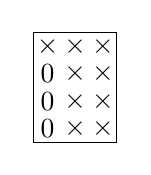
\begin{tikzpicture}[scale=0.35, baseline=-0.65ex]
    \draw (-1.5, -2) rectangle (1.5, 2);
    \node at (-1, 1.5) {$\times$}; \node at (0, 1.5) {$\times$}; \node at (1, 1.5) {$\times$};
    \node at (-1, 0.5) {$0$}; \node at (0, 0.5) {$\times$}; \node at (1, 0.5) {$\times$};
    \node at (-1, -0.5) {$0$}; \node at (0, -0.5) {$\times$}; \node at (1, -0.5) {$\times$};
    \node at (-1, -1.5) {$0$}; \node at (0, -1.5) {$\times$}; \node at (1, -1.5) {$\times$};
  \end{tikzpicture}.
\]
To do the next step, we need to be careful, since we don't want to destroy the previously created zeroes.

\begin{lemma}
  If the first $k - 1$ components of $\mathbf{u}$ are zero, then
  \begin{enumerate}
    \item For every $\mathbf{x} \in \R^m$, $H_{\mathbf{u}} \mathbf{x}$ does not alter the first $k - 1$ components of $\mathbf{x}$.
    \item If the last $(m - k + 1)$ components of $\mathbf{y} \in \R^m$ are zero, then $H_{\mathbf{u}}\mathbf{y} = \mathbf{y}$.
  \end{enumerate}
\end{lemma}
These are all obvious from definition. All these say is that reflections don't affect components perpendicular to $\mathbf{u}$, and in particular fixes all vectors perpendicular to $\mathbf{u}$.

\begin{lemma}
  Let $\mathbf{a}, \mathbf{b} \in \R^m$, with
  \[
    \begin{pmatrix}
      a_k\\
      \vdots\\
      a_m
    \end{pmatrix} \not=
    \begin{pmatrix}
      b_k\\
      \vdots\\
      b_m
    \end{pmatrix},
  \]
  but
  \[
    \sum_{j = k}^m a_j^2 = \sum_{j = k}^m b_j^2.
  \]
  Suppose we pick
  \[
    \mathbf{u} = (0, 0, \cdots, 0, a_k - b_k, \cdots, a_m - b_m)^T.
  \]
  Then we have
  \[
    H_\mathbf{u} \mathbf{a} = (a_1, \cdots, a_{k - 1} b_k, \cdots, b_m).
  \]
\end{lemma}
This is a generalization of what we've had before for $k = 1$. Again, the proof is just straightforward verification.

Now we can mess with the second column of $H_1 A$. We let $\mathbf{a}$ be the second column of $H_1 A$, and assume $a_3, \cdots, a_m$ are not all zero, i.e.\ $(0, a_2, \cdots, a_m)^T$ is not a multiple of $\mathbf{e}_2$. We choose
\[
  \mathbf{u} = (0, a_2 \mp \gamma, a_3, \cdots, a_m)^T,
\]
where
\[
  \gamma = \sqrt{\sum_{j = 2}^m a_j}.
\]
Then
\[
  H_\mathbf{u} \mathbf{a} = (a_1, \pm \gamma, 0, \cdots).
\]
Also, by the previous lemma, this does not affect anything in the first column and the first row. Now we have
\[
  H_2 H_1 A =
  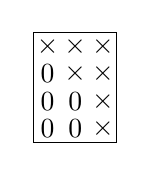
\begin{tikzpicture}[scale=0.35, baseline=-0.65ex]
    \draw (-1.5, -2) rectangle (1.5, 2);
    \node at (-1, 1.5) {$\times$}; \node at (0, 1.5) {$\times$}; \node at (1, 1.5) {$\times$};
    \node at (-1, 0.5) {$0$}; \node at (0, 0.5) {$\times$}; \node at (1, 0.5) {$\times$};
    \node at (-1, -0.5) {$0$}; \node at (0, -0.5) {$0$}; \node at (1, -0.5) {$\times$};
    \node at (-1, -1.5) {$0$}; \node at (0, -1.5) {$0$}; \node at (1, -1.5) {$\times$};
  \end{tikzpicture}
\]
Suppose we have reached $H_{k - 1} \cdots H_1 A$, where the first $k - 1$ rows are of the correct form, i.e.
\[
  H_{k - 1} \cdots H_1 A =
  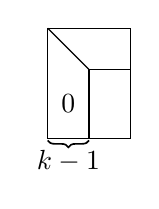
\begin{tikzpicture}[baseline=-0.65ex, scale=0.35]
    \draw (-1.5, -2) rectangle (1.5, 2);
    \draw (-1.5, 2) -- (0, 0.5);
    \draw (0, -2) -- (0, 0.5) -- (1.5, 0.5);
    \node at (-0.75, -0.75) {$0$};
    \draw [semithick, decorate, decoration={brace, mirror}, yshift=-2pt] (-1.5, -2) -- (0, -2) node [pos=0.5, below] {$k - 1$};
  \end{tikzpicture}
\]
We consider the $k$th column of $H_{k - 1} \cdots H_1 A$, say $\mathbf{a}$. We assume $(0, \cdots, 0, a_k, \cdots, a_m)^T$ is not a multiple of $\mathbf{e}_k$. Choosing
\[
  \mathbf{u} = \gamma(0, \cdots, 0, a_k \mp \gamma, a_{k + 1}, \cdots, a_m)^t,\quad \gamma = \sqrt{\sum_{j = k}^m a_j^2},
\]
we find that
\[
  H_\mathbf{u} \mathbf{a} = (a_1, \cdots, a_{k - 1}, \pm \gamma, 0, \cdots, 0)^T.
\]
Now we have
\[
  H_k \cdots H_1 A =
  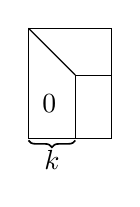
\begin{tikzpicture}[baseline=-0.65ex, scale=0.35]
    \draw (-1.5, -2) rectangle (1.5, 2);
    \draw (-1.5, 2) -- (0.2, 0.3);
    \draw (0.2, -2) -- (0.2, 0.3) -- (1.5, 0.3);
    \node at (-0.75, -0.75) {$0$};
    \draw [semithick, decorate, decoration={brace, mirror}, yshift=-2pt] (-1.5, -2) -- (0.2, -2) node [pos=0.5, below] {$k$};
  \end{tikzpicture},
\]
and $H_k$ did \emph{not} alter the first $k -1 $ rows and columns of $H_{k - 1} \cdots H_1 A$.

There is one thing we have to decide on --- which sign to pick. As mentioned, these do not matter in pure mathematics, but with inexact arithmetic, we should pick the sign in $a_k \mp \gamma$ such that $a_k \mp \gamma$ has maximum magnitude, i.e.\ $a_k \mp \gamma = a_k + \sgn(a_k) \gamma$. It takes some analysis to justify why this is the right choice, but it is not too surprising that there is some choice that is better.

So how do Householder and Givens compare? We notice that the Givens method generates zeros at one entry at a time, while Householder does it column by column. So in general, the Householder method is superior.

However, for certain matrices with special structures, we might need the extra delicacy of introducing a zero one at a time. For example, if $A$ is a band matrix, then it might be beneficial to just remove the few non-zero entries one at a time.
\end{document}
